\documentclass[fleqn,a4paper,12pt]{report}
\usepackage{graphicx}           % For adding pictures
\graphicspath{ {./images/} }    % Image folder to include from
\usepackage{anyfontsize}        % For setting exact font size
\usepackage{geometry}           % For setting margins
\geometry{a4paper, 
          left   = 35 mm, 
          right  = 25mm, 
          top    = 30mm, 
          bottom = 30mm}        % Margins according to Feri guidelines
\usepackage[utf8]{inputenc}     % For slovenian characters
\usepackage{sectsty}            % For setting font size of chapters 
\usepackage{titlesec}           % For setting the shape of chapters
\usepackage{lipsum}             % Lorem ipsum package for dummy text
\usepackage[parfill]{parskip}   % No indent
\usepackage{setspace}           % For 1 and half spacing between lines
\linespread{1.5}                % Look above
\usepackage{hyperref}           % Links
\usepackage{cite}               % Citations
\usepackage{url}                % Different links 
\usepackage[binary-units=true]{siunitx}
\usepackage{subcaption}         % Subcations for figures
\usepackage{amssymb}            % Additional symbols
\usepackage{listings}           % For code snippets
\usepackage[table]{xcolor}      % For color in code snippets and tables
\usepackage{dirtree}            % For printing directory trees
\usepackage{bigfoot}            % For code snippets in footnote texts
\usepackage{booktabs}           % For nicer tables
\usepackage{adjustbox}          % For rotating
\usepackage{rotating}           % Same as above
\usepackage{array}
\usepackage{xparse}             % http://ctan.org/pkg/xparse
\usepackage[super]{nth}         % For adding th to numbers
\usepackage{microtype}          % For converting from pdf to word
\DisableLigatures[Q,q,f,l,t,i]{}% Same as above
\usepackage{tabularx}           % Better tables

\setlength{\mathindent}{2cm}    % Indent equations 2cm from text edge
\setcounter{tocdepth}{4}        % Table of content goes to 4th level
\setcounter{secnumdepth}{4}     % Same here
\frenchspacing                  % One space after period dot
\interfootnotelinepenalty=10000 % Prevent automatic split of footnotes 

% Custom styling according to Feri guide lines
\def\poglavje{\fontsize{18}{18}\selectfont}
\def\podpoglavje{\fontsize{14}{18}\selectfont}
\def\podpodpoglavje{\fontsize{14}{18}\selectfont}
\def\podpodpodpoglavje{\fontsize{14}{18}\selectfont}

\titleformat{\chapter}[hang]
  {\poglavje\bfseries}{\thechapter }{0pt}{\poglavje}

\titleformat{\section}[hang]
  {\podpoglavje}{\thesection }{0pt}{\podpoglavje}

\titleformat{\subsection}[hang]
  {\podpoglavje}{\thesubsection }{0pt}{\podpodpoglavje}

\titleformat{\subsubsection}[hang]
  {\podpoglavje}{\thesubsubsection }{0pt}{\podpodpodpoglavje}


% Definitions for code formating and coloring
\definecolor{codegreen}{rgb}{0,0.6,0}
\definecolor{codegray}{rgb}{0.5,0.5,0.5}
\definecolor{codepurple}{rgb}{0.58,0,0.82}
\definecolor{backcolour}{rgb}{0.95,0.95,0.92}

\definecolor{backcolour}{rgb}{0.95,0.95,0.92}
\definecolor{tbgreen}{rgb}{0.50, 1, 0.36}
\definecolor{tbgreeny}{rgb}{0.8, 1, 0.54}
\definecolor{tbyellow}{rgb}{1, 0.9, 0.54}
\definecolor{tborange}{rgb}{0.87, 0.6, 0.11}
\definecolor{tbred}{rgb}{1, 0.68, 0.54}

\lstdefinestyle{mystyle}{
    backgroundcolor=\color{backcolour},   
    commentstyle=\color{codegreen},
    keywordstyle=\color{magenta},
    numberstyle=\tiny\color{codegray},
    stringstyle=\color{codepurple},
    basicstyle=\linespread{0.9}\ttfamily\footnotesize,
    breakatwhitespace=false,         
    breaklines=true,                 
    captionpos=b,                    
    keepspaces=true,                 
    numbers=left,                    
    numbersep=5pt,                  
    showspaces=false,                
    showstringspaces=false,
    showtabs=false,                  
    tabsize=2
}
% Change title of table of contents
\renewcommand{\contentsname}{Table of Contents}


% Add new rot command for rotating
\NewDocumentCommand{\rot}{O{45} O{1em} m}{\makebox[#2][l]{\rotatebox{#1}{#3}}}%

\begin{document}

%Zaključno delo, izdelano v tujem jeziku, mora vsebovati:
%• naslov zaključnega dela v tujem in slovenskem jeziku,
%• razširjen povzetek v slovenskem jeziku, ki mora po količini obsegati najmanj 5 %
%celotnega dela (od prvega do zadnjega poglavja, brez seznama virov ter prilog),
%•zaključno delo mora biti lektorirano s strani lektorja angleškega jezika.



% Mandatory parts of thesis, should delete later

% naslovna stran na platnici, tega ni v latex dokumentu
% • notranja naslovna stran v zaključnem delu,
% done

% • naslednja notranja naslovna stran
% nevem če je pravi naziv za krambergerja in vojislava preveri

% • zahvala
% layout ok, so problemi če je preveč teksta, dejansko še moraš napisati zahvalo.  
% • stran z naslovom, ključnimi besedami, UDK [1] klasifikacijo in povzetkom
% zaključnega dela v slovenskem jeziku,
% • stran z naslovom, ključnimi besedami, UDK 1 klasifikacijo in povzetkom zaključnega
% dela v angleškem jeziku,
% Izgleda ok, potrebno je dopolniti
% • kazalo vsebine,
% • kazalo slik,
% • kazalo grafov
% • kazalo tabel,
% • seznam uporabljenih simbolov in kratic,
% • vsebina zaključnega dela,
% • seznam uporabljenih virov in literature,
% • priloge k zaključnemu delu,
% • izjava o avtorstvu in istovetnosti tiskane in elektronske oblike zaključnega dela v
% trdo vezanem izvodu (v preostalih izvodih naj bo fotokopija),


%\pagenumbering{gobble}
%\begin{titlepage}
    \begin{center}
 
        \fontsize{16}{26}
        \selectfont
        UNIVERZA V MARIBORU\\
        FAKULTETA ZA ELEKTROTEHNIKO,\\
        RAČUNALNIŠTVO IN INFORMATIKO
        \vspace*{3.0cm}

        \textbf{Marko Sagadin}

        \vspace{0.5cm}

        \fontsize{26}{26}
        \selectfont
        \textbf{Energy efficient system for detection of elephants with machine learning}
 
        \vspace{1.0cm}

        \fontsize{26}{26}
        \selectfont
        \textbf{Energetsko učinkovit sistem za detekcijo slonov s pomočjo strojnega učenja}

        \vspace{0.5cm}

        \fontsize{16}{18}
        \selectfont
        Master's thesis
 
        \vspace*{\fill}

        Maribor, May 2020 
 
 
    \end{center}
\end{titlepage}
          % We repeat this twice, first for the cover
%\begin{titlepage}
    \begin{center}
 
        \fontsize{16}{26}
        \selectfont
        UNIVERZA V MARIBORU\\
        FAKULTETA ZA ELEKTROTEHNIKO,\\
        RAČUNALNIŠTVO IN INFORMATIKO
        \vspace*{3.0cm}

        \textbf{Marko Sagadin}

        \vspace{0.5cm}

        \fontsize{26}{26}
        \selectfont
        \textbf{Energy efficient system for detection of elephants with machine learning}
 
        \vspace{1.0cm}

        \fontsize{26}{26}
        \selectfont
        \textbf{Energetsko učinkovit sistem za detekcijo slonov s pomočjo strojnega učenja}

        \vspace{0.5cm}

        \fontsize{16}{18}
        \selectfont
        Master's thesis
 
        \vspace*{\fill}

        Maribor, May 2020 
 
 
    \end{center}
\end{titlepage}
          % page, then for the first inside page
%\begin{center}

    \vspace*{4.0cm}
    \fontsize{26}{26}
    \selectfont
    \textbf{Energy efficient system for detection of elephants with machine learning}

    \vspace{1.0cm}

    \fontsize{26}{26}
    \selectfont
    \textbf{Energetsko učinkovit sistem za detekcijo slonov s pomočjo strojnega učenja}

    \vspace{0.5cm}

    \fontsize{16}{18}
    \selectfont
    Master's thesis

\end{center}

\vspace*{\fill}

\begin{tabular}{ l l }
    Student: & Marko Sagadin  \\ 
    Study program: & Second Cycle Bologna Study Programme of\\  
                   & Electrical Enigneering \\
    Module of study program: & Electronics \\
    Mentor: & doc. dr. Iztok Kramberger univ. dipl. inž. el. \\
    Co-mentor: & Mag. nekaj nekaj Vojislav Dragan Milivojević \\
\end{tabular}

\newpage


%\pagenumbering{roman}
%\begin{poglavje}
\noindent\bfseries Zahvala
\end{poglavje}

To magistrsko delo ne bi bilo možno brez pomoči nekaterih ljudi.
Prvo bi se rad zahvalil mentorju Iztoku Krambergerju in somentorju Vojislavu Draganu Milivojeviču za njune neprecenljive nasvete in napotke.
Posebej bi se rad zahvalil Luki Mustafi, mojemu šefu in nenapisanemu mentorju.
Hvala ti za nasvete, za mnoge sestanke, da si skrbel, da je napisano dosegalo visoke standarde in za vedno prižgan AWS server.
Rad bi se zahvalil mojim sodelavcem na Irnasu za njihovo podporo, še posebej mojima prijateljema Nejcu in Vidu, da sta si vzela čas in pregledala mojo delo.

Rad bi se zahvalil Arribadi Initiative, ki je priskrbela nabor termalnih slik in tako sploh omogočila nastanek tega dela.
Hkrati bi se tudi rad zahvalil Danileu Situnayakeju in Janu Jongboomu, za odgovore na vsa moja vprašanja v zvezi s TinyML-om.

Rad bi se zahvalil mojim staršem za njihovo podporo in spodbudo skozi vsa leta mojega šolanja.
Brez vaju dveh ne bi bil tukaj, kjer sem sedaj.

Nazadnje se želim zahvaliti moji punci Hristini, ker je verjela vame in me podpirala med pisanjem magistrskega dela.
\clearpage

\begin{poglavje}
\noindent\bfseries Acknowledgement
\end{poglavje}

This Master's thesis would not be possible without the assistance of certain people.
Firstly, I would like to thank Mentor Iztok Kramberger and Co-mentor Vojislav Dragan Milivojević for their invaluable guidance and feedback.
Special thanks go to Luka Mustafa, my boss and unwritten mentor.
Thank you for your advice, for numerous feedback sessions, for making sure that the writing is up to a high standard and for the 24/7 AWS server.
I would like to thank my colleagues at Irnas for their support, especially my friends Nejc and Vid, for taking the time to read and correct my work.

I want to thank the Arribada Initiative for providing me with the thermal image dataset, thus making this thesis possible in the first place.
Additionally I would like to thank Daniel Situnayake and Jan Jongboom, for answering all my TinyMl related questions.

I want to thank my parents for supporting and encouraging me through the years of my education. 
Without you, I would not be here, where I am today.

Lastly I want to thank my girlfriend Hristina for believing in me and supporting me during thesis writing.
\newpage

\begin{poglavje}
\noindent\bfseries Energetsko učinkovit sistem za detekcijo slonov s pomočjo strojnega učenja
\end{poglavje}

\bigskip
\bigskip
\bigskip
\bigskip
\bigskip
\textbf{Ključne besede:} strojno učenje, mikrokrmilnik, sklepanje na napravi, termalna kamera, sistem z majhno porabo, 
\bigskip
\textbf{UKD:} XXXXX

\bigskip
\bigskip
\bigskip
\bigskip
\textbf{Povzetek}

\lipsum[1-5]
\newpage

\begin{poglavje}
\noindent\bfseries Energy efficient system for detection of elephants with Machine Learning
\end{poglavje}

\bigskip
\bigskip
\bigskip
\bigskip
\bigskip
\textbf{Key words:} machine learning, microcontroller, on-device inference, thermal camera, low-power system

\bigskip
\textbf{UKD:} XXXXX

\bigskip
\bigskip
\bigskip
\bigskip
\textbf{Abstract}

Human-Elephant Conflicts are a major environmental and animal conservative problem, according to WILDLABS, because of it an average of 400 people and 100 elephants are killed every year in India alone. 
Early warning systems could replace the role of human watchers and warn local communities of nearby, potentially life threatening, elephants, thus minimising the Human-Elephant Conflicts.

In this Master's thesis we present the structure of an early warning system, which consists of several deployed embedded systems equipped with thermal cameras and a single gateway; the main focus of the thesis was the design and implementation of the former.
To detect presence of elephants, we designed and trained several accurate image classification models, capable of classifying thermal images.
We optimised said models for on-device performance and compared them in terms of accuracy, execution speed and size.
While writing firmware we ported a part of TensorFlow library and created our own build system, suitable for the platform of our choice. 
We also implemented reporting of inference results over LoRaWAN network and described possible server-size setup.
We finally constructed fully functional embedded system from various development and evaluation boards, and evaluated its performance in terms of inference speed and power consumption.
We show that embedded systems with Machine Learning capabilities are a viable solution to many real life problems.
\newpage


%\tableofcontents
%\listoffigures
%\listoftables


%\chapter{ Introduction}
%\pagenumbering{arabic}
%\section{ Motivation}

Elephants are dangerous and smart animals.\cite{scientificelephant}

Wild Lab claims:
In India alone, an average of 400 people and 100 elephants are killed every year as a result of human-wildlife conflict. 

Wild Lab
In Northeast-India, human elephant conflicts are increasingly common. Electric fences were developed to prevent elephants from entering villages and crop fields.

Elephants are intelligent animals and will eventually always find ways to break fences and enter crop fields. For example, tuskers learn how to break wires and poles with their tusks and elephants have been observed throwing logs and other tools on the wires.  Currently, to identify damaged fences and to understand how this happened, camera traps with motion sensors can be deployed. They send warning messages or trigger an alarm. However, camera traps are costly and their passive lasers can’t differentiate between elephants and other wildlife (or people) and are thus constantly triggered by any movement

Early detection of elephants will prevent surprise encounters and will give people more time to choose the best response to prevent escalation into conflict. Existing early detection tools can only detect elephants at short distances


What is causing the Human-Elephant Conflict problem

    Steady degradation of habitat due to encroachment and an increasing human population
    Habitat loss due to land-use change resulting from encroachment, agriculture and infrastructure development
    Disruption of wildlife corridors
    Habitat degradation due to over-extraction and weed infestation (causing elephants to look for better fodder in cultivated fields) and monoculture plantations

What conflicts occur

    Crop raids
    Damage to property
    Human fatalities and injuries
    Elephant fatalities (accidental electrocution or poisoning)
    Retaliatory killings of elephant
        Describe the problem, role of IRNAS, Arribada and Smart parks, write about current solutions, power hungry raspi, proposed solution, "The goal of this dissertation project is to...", should be 2-3 pages long, a nice story.
fdlsdjfsf

%
%\chapter{ Theoretical description of system building blocks}
%\section{ Machine learning}

According to Arthur Samuel (qtd. in Geron \cite{geron}) machine learning is a field of study that gives computers the ability to learn without being explicitly programmed.
This ability to learn is the property of various machine learning algorithms.
We will be using terms "machine learning" and "learning" interchangeably. 
In order to learn, these learning algorithms need to be trained on a collection of examples of some phenomenon\cite{burkovml}. 
These collections are called \textbf{datasets} and can be generated artificially or collected in nature.

In order to better understand how ML approach can solve problems, we can examine an example application.
Let us say that we would like to build a system that can predict a type of animal movement from an accelerometer data.
To train its learning algorithm, also known as a \textbf{model}, we need to expose it to a dataset which would contain accelerometer measurements of different types of movement, such a walking, running, jumping and standing still.
Input to the system could be either raw measurements from all three axis or components extracted from raw measurements such as frequency or amplitude. 
These inputs are also known as \textbf{features}, they are values that describe the phenomenon being observed\cite{burkovml}. 
The output of the system would be a predicted type of movement.
Although we would mark each example of measurement data what type of movement it represents, we would not directly define the relationship between the two.
Instead, we would let the model figure out connection by itself, through the process of training.
The trained model should be general enough so it can correctly predict the type of movement on unseen accelerometer data.

There exists a large variety of different learning algorithms. 
We can broadly categorize them in several ways, one of them depends on how much supervision learning algorithm needs in the training process. 
Algorithms like K-nearest neighbours, linear and logistic regression, support vector machines fall into the category of supervised learning algorithms.
Training data that is fed into them includes solutions, also known as \textbf{labels}\cite{geron}.
Described above example is an example of a supervised learning problem.

Algorithms like k-Means, Expectation Maximization, Principal Component Analysis fall into the category of unsupervised learning algorithms.
Here training data is unlabeled, algorithms are trying to find similarities in data by itself\cite{geron}.
There exist other categories such as semi-supervised learning which is a combination of previous two and reinforcement learning, where model acts inside environment according to learned policies\cite{geron}.

Neural networks, algorithms inspired by neurons in human brains\cite{geron}\cite{cs231n}, can fall into either of categories. 
They are appropriate for solving complex problems like image classification, speech recognition, and autonomous driving, but they require a large amount of data and computing power for training.
They fall into field of deep learning, which is a sub-field of machine learning.

Training of deep learning algorithms is computationally demanding and is usually done on powerful servers or computers with dedicated graphic processing units to speed up training time.
After a model has been trained, data can be fed in and prediction is returned. 
This process is also known as \textbf{inference}.
The inference is computationally less intensive compared to the training process, so with properly optimised models, we can run inference on personal computers, smartphones, tablets, and even directly in internet browsers.


\subsection{ General machine learning workflow}

There are several steps in ML workflow that have to occur in order to get from an idea to a working ML based system as seen on Figure \ref{ml_workflow}.

\begin{figure}[ht]
        \centering
        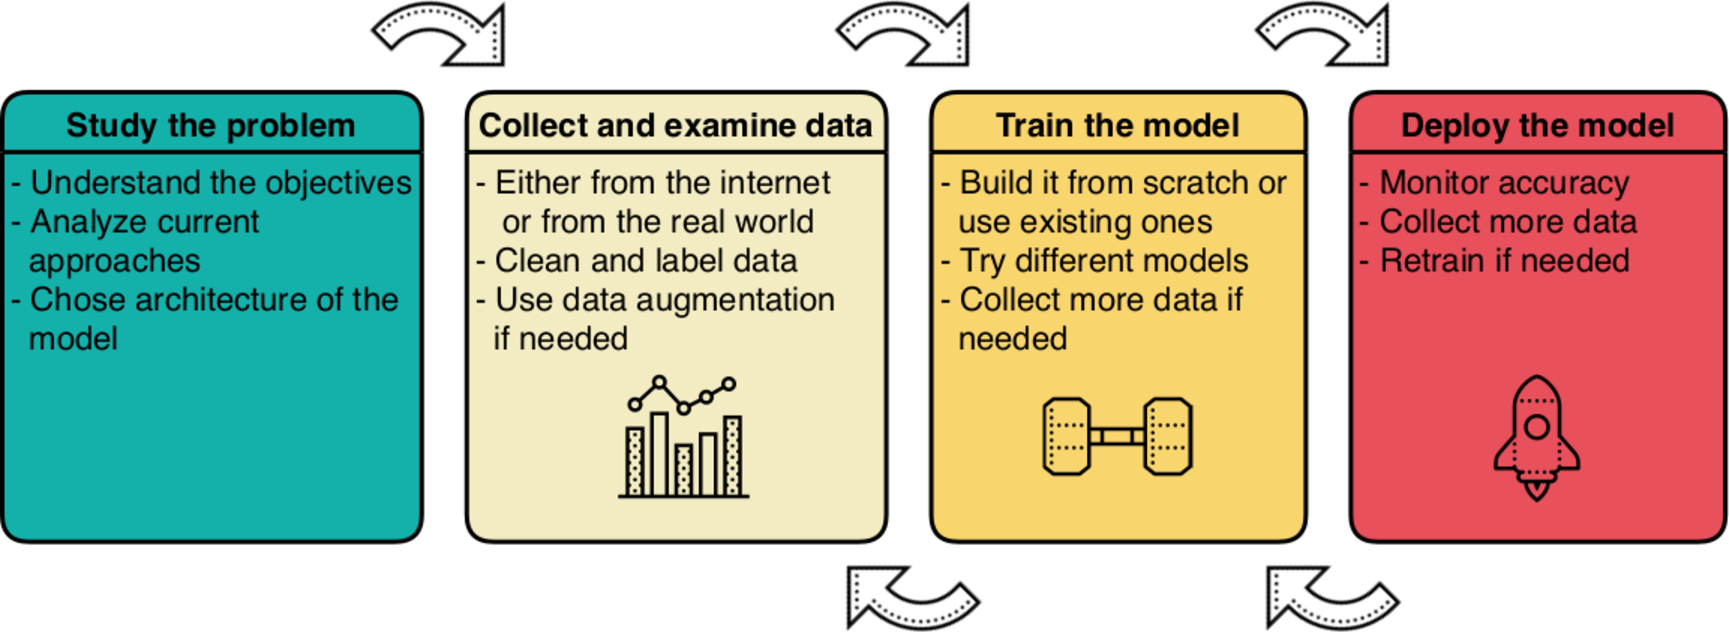
\includegraphics[width=1.0\linewidth]{ml_workflow.pdf} 
        \caption{ Workflow of solving a generic machine learning problem. Icons source: www.icons8.com}
        \label{ml_workflow}
\end{figure}

First problem has to be studied, it has to be understood what are objectives and decided which approach will be used. 
Here we decide on rough architecture of the ML model that we will use.
In second step we collect and clean up data.
We should always strive to collect large amount of quality and diverse data that represents real word phenomenon.
Collecting that kind of data can be hard and expensive, but we can use various tools of for producing synthetic data from our original data, thus increasing data size and variety.
Third, we train ML model.
We might create something from scratch or use an existing model. 
We can train several different types of models and chose the one that performs the best.
To achieve desired accuracy, steps two and three can be repeated many times.
In step four we deploy our model and monitor its accuracy. We can also use it to collect more data and retrain the model.


\subsection{ Machine learning on embedded devices} \label{ml_on_embedded}

Machine learning on embedded devices is an emerging field, which nicely coincides with the Internet of things.
Resources about it are limited, especially when compared to the wast number of resources connected with machine learning on computers or servers.
Most of the information about it can be found in form of scientific papers, blog posts and machine learning framework documentation\cite{hello_edge}\cite{tflite_risc-v}\cite{pete_tiny}.

Running learning algorithms directly on smart devices comes with many benefits.
One of them is reduced power consumption.
In most IoT applications devices send raw sensor data over a wireless network to the server, which processes it either for visualization or for making informed decisions about the system as a whole. 
Wireless communication is one of the more power hungry operations that embedded devices can do, while computation is one of more energy efficient\cite{pete_tiny}.
For example, a Bluetooth communication might use up to 100 milliwatts, while MobileNetV2 image classification network running 1 inference per second would use up to 110 microwatts\cite{pete_tiny}
As deployed devices are usually battery powered, it is important to keep any wireless communication to a minimum, minimizing the amount of data that we send is paramount.
Instead of sending everything we capture, is much more efficient to process raw data on the devices and only send results.

Another benefit of using ML on embedded devices is decreased time between event and action.
If the devices can extract high-level information from raw data, they can act on it immediately, instead of sending it to the cloud and waiting for a response. 
Getting a result now takes milliseconds, instead of seconds.

Such benefits do come with some drawbacks.
Embedded devices are a more resource constrained environment when compared to personal computers or servers.
Because of limited processing power, it is not feasible to train ML models directly on microcontrollers.
Also it is not feasible to do online learning with microcontrollers, meaning that they would learn while being deployed.
Models also need to be small enough to fit on a device. 
Most general purpose microcontrollers only offer several hundred kilobytes of flash, up to 2 megabytes.
For comparison, MobileNet v1 image classification model, optimised for mobile phones, is 16.9 MB in size\cite{daniel_edgeimpulse}.
To make it fit on a microcontroller and still have space for our application, we would have to greatly simplify it.

Usual workflow, while developing machine learning models for microcontrollers, is to train a model on training data on a computer. 
When we are satisfied with the accuracy of the model we then quantize it and convert it into a format understandable to our microcontroller.
This is further described in section \ref{tflite_quant}.
%This workflow is described in section \ref{tflite_quant} in greater detail.

\section{ Neural networks}\label{neural_networks_section}

Although first models of neural networks (NN) were presented in 1943 (by McCulloch and Pitts)\cite{geron} and hailed as the starting markers of the artificial intelligence era, it had to pass several decades of research and technological progress before they could be applied to practical, everyday problems.
Early models of NNs, such as the one proposed by McCulloch and Pitts were inspired by how real biological neural systems work. 
They proved that a very simple model of an artificial neuron, with one or more binary inputs and one binary output is capable of computing any logical proposition when used as a part of a larger network\cite{geron}.

To learn how NNs work we can refer to Figure \ref{neuron_model}, which shows a generic version of an artificial neuron.
\newline

\begin{figure}[ht] 
    \begin{subfigure}[b]{0.5\textwidth}
        \centering
        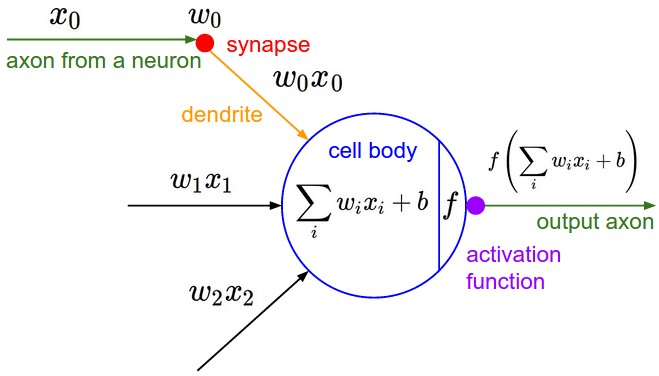
\includegraphics[width=1.0\linewidth]{neuron_model.jpeg} 
        \caption{Artificial neuron}
        \label{neuron_model}
    \end{subfigure}
    \unskip\ \vrule\ 
    \begin{subfigure}[b]{0.5\textwidth}
        \centering
        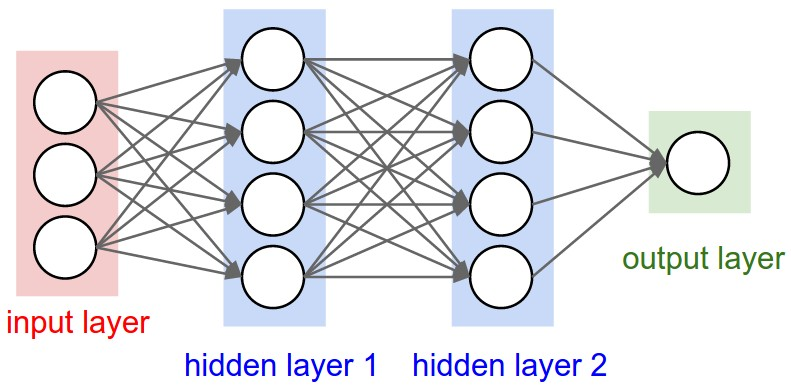
\includegraphics[width=1.0\linewidth]{neural_net.jpeg} 
        \caption{ 3-layer neural network}
        \label{neural_net}
    \end{subfigure}
    
    \caption{ (a) Mathematical model of an artificial neuron, similarities with biological neurons can be seen. (b) Fully connected 3-layer neural network. Image source: \cite{cs231n}}
    \label{neural}
\end{figure}

Neuron takes several inputs, multiplies each input with its \textbf{weight} and sums them up.
It adds to the sum the \textbf{bias} term and then applies an activation function.

NNs consist of many neurons, which are organized into \textbf{layers}.
Neurons inside the same layer do not share any connections, but they connect to layers before and after them.
First layer is known as \textbf{input} layer and last one is known as \textbf{output} layer. 
Any layers between are said to be \textbf{hidden}. 
On Figure \ref{neural_net} we can see neural network with an input layer with three inputs, two hidden layers with four neurons each and a output layer with just one neuron.
If all inputs of neurons in one layer are connected to all outputs from previous layer, we say that a layer is \textbf{fully connected} or \textbf{dense}, Figure \ref{neural_net} is an example of one.
NNs with many hidden layers fall into category of deep neural networks (DNN).


\subsection{ Activation functions}

Activation functions introduce non-linearity to chain of otherwise linear transformations, which enables ANNs to approximate any continuous function\cite{geron}.
There are many different kinds of activation functions as seen on Figure \ref{activation_functions}, such as sigmoid function and rectified linear activation function (ReLu).
Sigmoid function was commonly used in the past, as it was seen as a good model for a firing rate of a biological neuron: 0 when not firing at all and 1 when fully saturated and firing at maximal frequency\cite{cs231n}.
It basically takes a real number and squeezes it into range between 0 and 1.
It was later shown that training NNs with sigmoid activation function often hinders training process as saturated outputs cut of parts of networks, thus preventing training algorithm reaching all neurons and correctly configuring the weights\cite{cs231n}.
It has since fallen out of practice and is nowadays replaced by ReLu or some other activation function.

\begin{figure}[ht!]
        \centering
        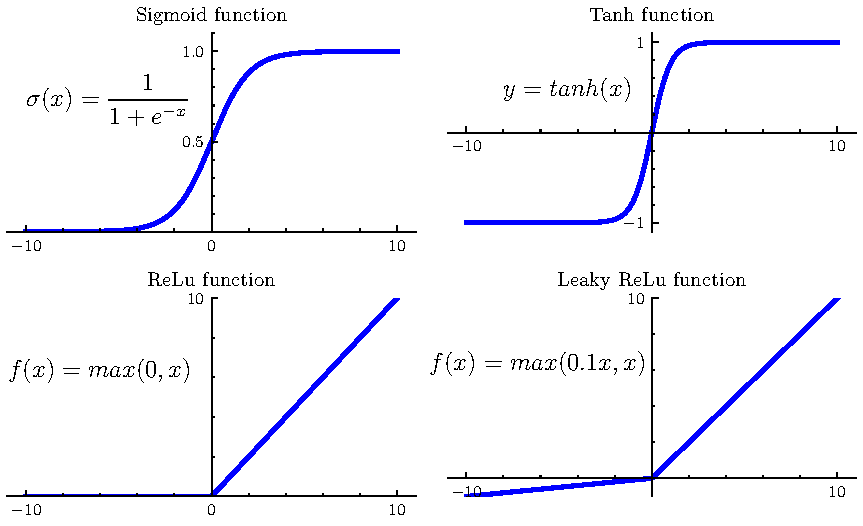
\includegraphics[width=1.0\linewidth]{activation_func.pdf} 
        \caption{Different activation functions and their equations.}
        \label{activation_functions}
\end{figure}


\subsection{ Backpropagation}

Training of neural networks is done with a training algorithm, known as \textbf{backpropagation}.
As mentioned before, we train the neural network by showing it a large amount of training data with labels.
At the start of the training phase, all weights and biases are set to randomly small values.
During each training step neural network is shown a small batch of training data. 
Each instance is feed into NN and final output label is calculated.
This is known as \textbf{forward pass}, which is exactly the same as making predictions, except that intermediate results from each neuron in every layer are stored.
Calculated output is compared to an expected one using a \textbf{loss} (also known as \textbf{cost}) function.
Loss function returns a single value, which tells us how badly is our NN performing, higher it is, worse is our NN performing.
The goal is to minimize the loss function, thus increasing the accuracy of our NN.
In the context of multivariable calculus this means that we have to calculate negative gradient of weights and biases which will tell us in which direction we have to change each weight and bias so that value of loss function decreases. 

Doing this for all weights and biases at the same time would be complicated, so backpropagation algorithm does this in steps.
After computing loss function algorithm analytically calculates how much each output connection contributed to loss function (essentially local gradient) with the help of previously stored intermidiate values.
This step is recursively done for each layer until first input layer is reached.
At that moment algorithm knows in which direction should each weight and bias change so that value of loss function lowers.
Procedure known as \textbf{Gradient Descent} is then performed.
All local gradients are multiplied with a small number known as \textbf{learning rate} and then subtracted from all weights and biases.
This way in each step we slowly change weights and biases in the right direction, while minimizing loss function.
Gradient Descent is not only used when training neural networks, but also when training other ML algorithms.

We do not have to execute backpropagation algorithm for each training instance, instead we can calculate predictions for a small set of training data, calculate average loss function and then apply backpropagation.


\subsection{ Convolutional neural networks}

Convolutional neural networks (CNN) are a kind of neural networks that work specially well with image data.
Like NNs they have found inspiration in nature, in their case visual cortex of the brain\cite{geron}.
It was shown that different cells in visual cortex responded differently to different visual stimuli\cite{cs231n}.
Some were activated when shown a horizontal line in specific location, some were activated by vertical lines.
More complex cells responded to boxes, circles and so on.
CNNs also detect simpler shapes first and use them to detect more complex ones later.

On Figure \ref{convnet} we can see an example of CNN which takes an image of a car as a input and outputs probability results in five different classes.
\newline

\begin{figure}[ht]
        \centering
        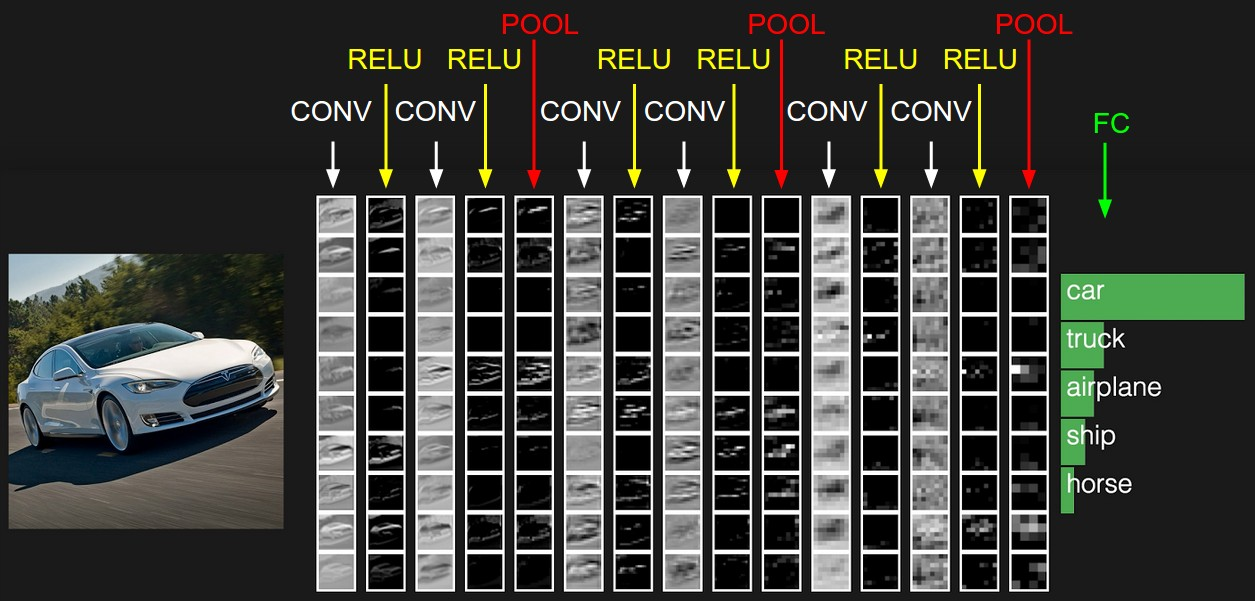
\includegraphics[width=1.0\linewidth]{convnet.jpeg} 
        \caption{CNNs usually consist of alternating convolutional layers and pooling layers. Last polling layer is flattened out and feed into fully connected NN. Image source:\cite{cs231n}}
        \label{convnet}
\end{figure}

Specific to CNNs are two different types of layers, \textbf{convolutional} layers and \textbf{pooling} layers.
Each convolutional layer detects some sort of shapes, first ones detect different kinds of edges, later ones detect more complex shapes and objects, like wheels, legs, eyes, ears.
Pooling layers downsample the data in spatial dimension, thus decreasing the number of parameters and operations needed in CNN.
After few alternating pairs of convolutional and pooling layers the output of the last pooling layer is flattened out into one dimensional vector and feed into fully connected NN which produces probability results in given classes.

It makes sense to explain how convolutional and pooling layers work in greater detail as this will be important later when we will be designing our CNN models in section TODO.


\subsubsection{ Convolutional layers}

Data that CNNs operate on are 3 dimensional matrices, where width and height correspond to image resolution and depth corresponds to the number of color channels, 3 for colorful images (red, green, blue) and 1 for greyscale.
When speaking about this data we will relate to them as volumes.

Convolution layers perform dot products between input volume and several \textbf{filters} or \textbf{kernels} to produce output volume.
In these layers filters are being configured through training phase.
We can see a concrete example on Figure \ref{conv1}.
2D filter with size 2 x 2 covers part of input volume, element-wise multiplication is computed, elements are summed and result is written into first element of output volume.

\begin{figure}[ht] 
    \centering
    \begin{subfigure}[b]{0.75\textwidth}
        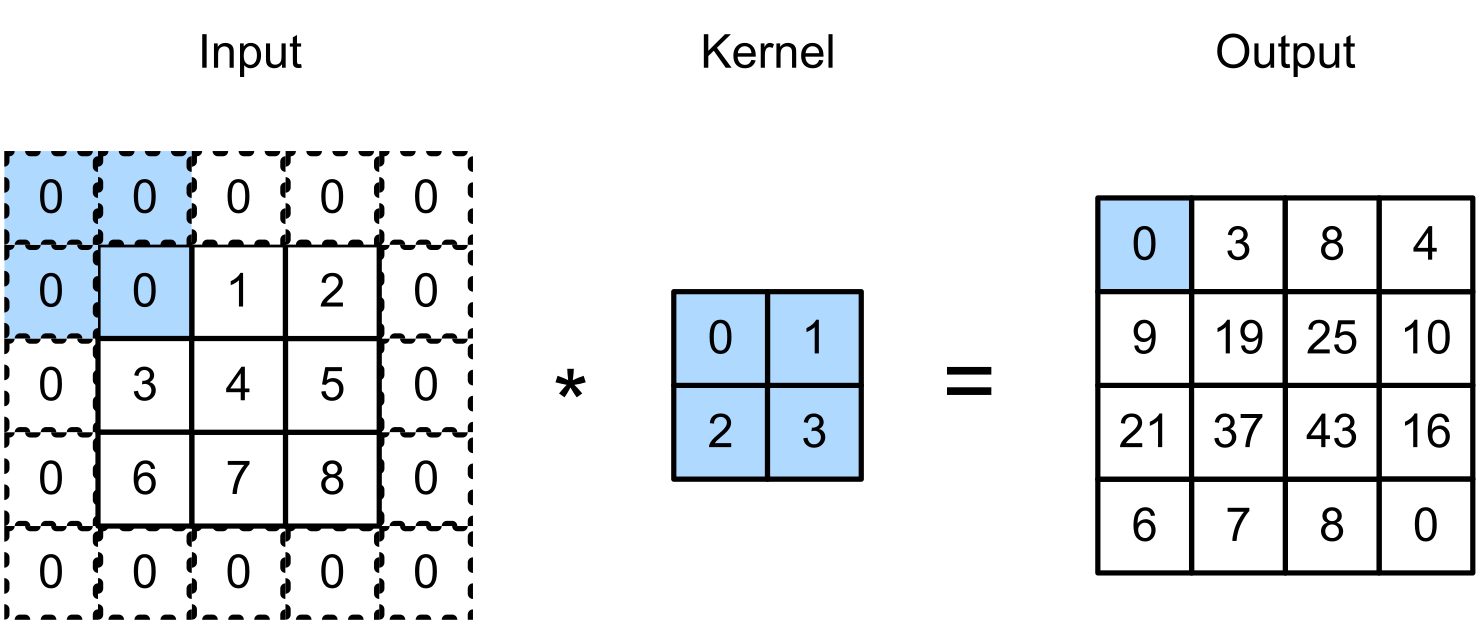
\includegraphics[width=\linewidth]{conv1.png} 
        \caption{Example of a dot product operation}
        \label{conv1}
    \end{subfigure}
    \vspace{0.5cm}
    \hrule
    \vspace{0.5cm}
    \begin{subfigure}[b]{0.5\textwidth}
        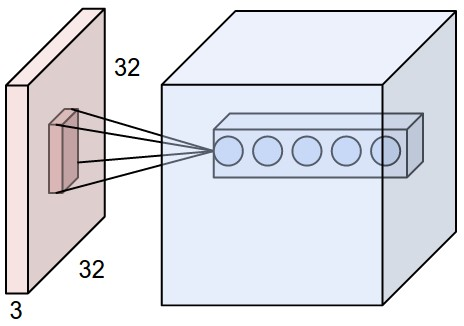
\includegraphics[width=\linewidth]{conv2.jpeg} 
        \caption{ Convolutional layer}
        \label{con2v}
    \end{subfigure}
    
    \caption{ (a) Filter moves over zero-padded input matrix. (b) To produce output layer with depth 5, this layer would have 5 different filters. Image sources: \cite{conv_layer_img}\cite{cs231n}}
    \label{conv_layer}
\end{figure}

Filter then moves a fixed width or \textbf{stride} and process is repeated.
It is important to note that although we can choose width and height of filter, depth of filter is always equal to the depth of the input volume.
If depth is larger than one then dot products are done for each 2D matrix in depth dimension separately and then element-wise sum between these matrices is performed.
To avoid loosing information from the image pixels that are on the edges (as they would be included in dot products less times compared to central ones) we often pad input images with zeros.

The size of output volume depends on several factors as seen in \ref{size_eq}.

\begin{equation}\label{size_eq}
V_{o} = (V_{i} - F + 2P) / S + 1
\end{equation}

Where:

$V_{i}$ - Input volume size, only width or height

$V_{o}$ - Output volume size, only width or height

$F$ - Filter or receptive field size

$P$ - Amount of zero padding used on the border

$S$ - Stride length

If we examine example on Figure \ref{conv1} we can see that input with a size 3 x 3, stride 1, padding 1 and filter with a size 2 x 2 produces output with size a 4 x 4.

Depth of output volume is equal to the number of filters used in convolutional layer, it is a norm that a single convolutional layer uses large number of filters to produce a deep output volume\cite{cs231n}.
It is also common to set padding, stride and filter size so that width and height of input volume are preserved.
This prevents the information at the edges to be lost too quickly\cite{cs231n}.

In the end of convolutional layer output volume is fed into neuron similar to one described in section \ref{neural_networks_section}. 
All elements in same depth are affected by a same bias term and fed into activation function.
In this step size of volume is preserved.

\subsubsection{ Pooling layers}

Polling layers perform downsampling of input volumes in width and height dimensions.
This is done by sliding a filter of fixed size over input and doing MAX operation on elements that filter covers, only the largest value element is copied into output (Figure \ref{pool_layer}).
Pooling is done on each depth slice separately of other slices, so depth size is preserved through the layer.

\begin{figure}[ht] 
    \begin{subfigure}[b]{0.5\textwidth}
        \centering
        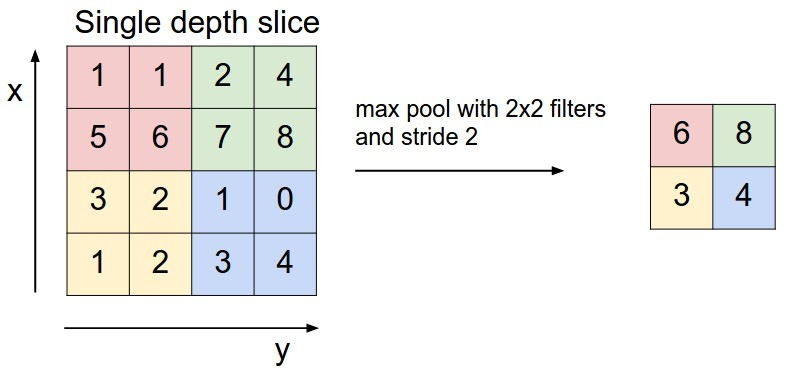
\includegraphics[width=1.0\linewidth]{pool1.jpeg} 
        \caption{Max pooling operation}
        \label{pool1}
    \end{subfigure}
    \unskip\ \vrule\ 
    \begin{subfigure}[b]{0.5\textwidth}
        \centering
        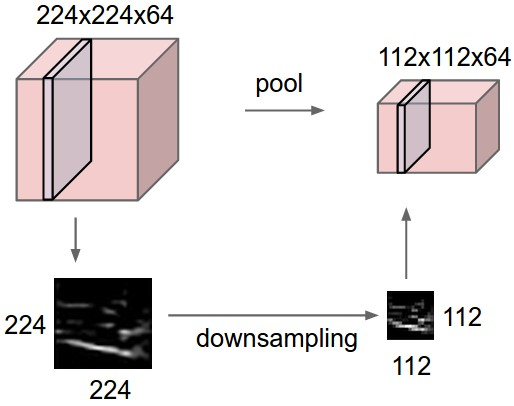
\includegraphics[width=1.0\linewidth]{pool2.jpeg} 
        \caption{ Effect of polling on input dimensions}
        \label{pool2}
    \end{subfigure}
    \caption{ Polling layer. Image source: \cite{cs231n}}
    \label{pool_layer}
\end{figure}

It is common to select pool size 2 x 2 and stride 2.
Like this inputs are downsampled by two in height and width dimensions, discarding 75 \% activations.
Pooling layers therefore reduce number of activations and prepare them to be flattened out and fed into fully connected layer.

\section{ TensorFlow}

TensorFlow is a free and open-source framework for numerical computation.
It is particularly suited for large-scale machine learning applications\cite{geron}.
TensorFlow started as a proprietary project developed by a Google Brain team at Google in 2011 and became open-source in late 2015.
It is used in many Google's products such as Gmail, Google Cloud Speech and Google Search.

TensorFlow gives programmers tools for creating and training ML models, without needlessly diving into specifics of computing neural networks.
Programmers can write high level code in Python API, which calls highly efficient C++ code.
When using TensorFlow the hardest part of a ML project is usually data preparation.
After that is done, the creation of a ML model, its training and evaluation can be done in a few lines of Python code.

TensorFlow also supports Keras high level API for building ML models. 
Keras is a Python library that functions as a wrapper for TensorFlow.
When building ML models developers can use Keras Sequential API, where each layer in a model is represented as one line of code.
Users do not need to care about connections between the layers, they only need to choose the type of layer (convolutional, max pool, fully connected), its size and few other specific parameters.
Sequential API is used most of the time, if finer level of control is needed TensorFlow provides low level math operations as well.

And finally, TensorFlow's trained output model is portable\cite{geron}.
Models can be trained in one environment and executed in another.
This means that we can train our model by writing Python code on Linux machine and execute it with Java on Android device.
This last functionality is important for running ML models on microcontrollers.

\subsection{ TensorFlow Lite for Microcontrollers} \label{tflite_quant}

TensorFlow Lite (TFLite) is a set of tools and libraries that enable running ML inferences on constrained devices\cite{tensorflow_github}.
It provides support for Android and iOS devices, and embedded Linux.
TensorFlow Lite for Microcontrollers (TFLite Micro) is a recent port of TFLite (as of mid 2019), dedicated to running ML models on microcontrollers.
TFLite itself provides API in different languages, such as Java, Swift, Python and C++.
TFLite Micro uses C++ API, specifically C++11, which reuses large part of the general TensorFlow codebase.

TFLite Micro library does not require any specific hardware peripherals, which means that the same C++ code can be compiled to run on a microcontroller or a personal computer with minimal changes.
Users are only expected to implement their own version of \verb|printf()| function.
As microcontroller binaries are usually quite big, flashing firmware to a microcontroller is a time consuming procedure.
It makes sense to first test and debug the program that includes only ML inference specific code on a personal computer, before moving on to a microcontroller in order to save time.
Implementation of test setup is described in TODO ADD REFERENCE.

TFLite Micro library is publicly available as a part of a much larger TensorFlow project on GitHub\cite{tensorflow_github}.
To use the library for embedded development the whole project has to be cloned from the GitHub.
TensorFlow team provides users with several example projects that have been ported to several different platforms such as Mbed, Arduino, OpenMV and ESP32.
Example projects show how to use TFLite API while showcasing different ML applications: motion detection, wake word detection and person detection.

Part of this thesis was concerned with porting TFLite Micro to \textbf{libopencm3}, our platform of choice.
To compile source files and build binaries TFLite Micro uses build automation tool \textbf{GNU Make}.
One large makefile that includes several platform specific makefiles dictates how firmware is built.
By providing command line arguments users decide which example has to be compiled and for which platform.
The build system makes some assumptions about locations of the platform specific files, which in case of example projects are scattered over GitHub repository.
This and several other reasons make library hard to use when porting it to a new platform.
In section TODO ADD REFERENCE we describe our build system that keeps library and application specific code separated in a clear and concise manner.

Is important to know that TFLite is just an extension of existing TensorFlow project.
General steps for creating a trained ML model are still the same as seen in Figure \ref{ml_workflow}, although we have to be aware of some details.
Figure \ref{micro_workflow} shows all steps that are needed to prepare a ML model for running on a microcontroller.

\begin{figure}[ht] 
    \centering
    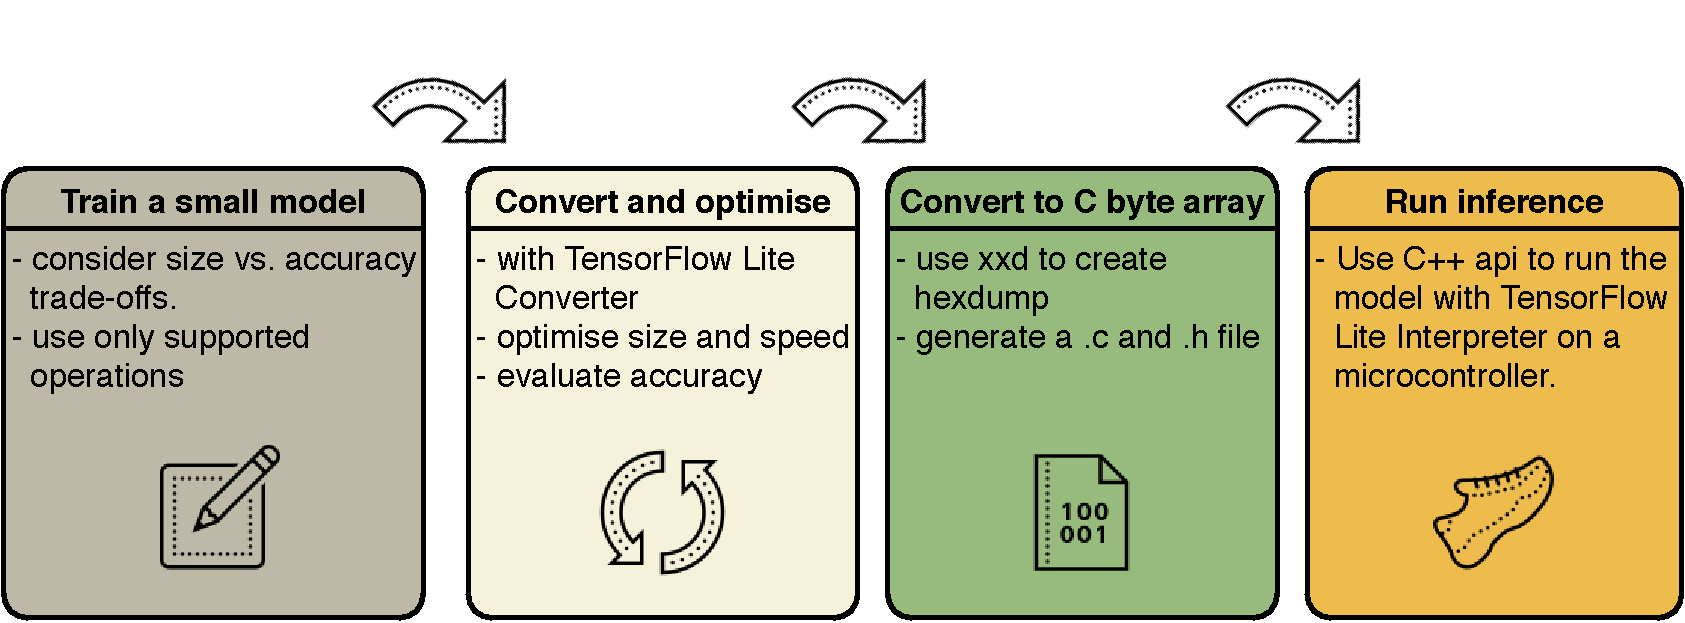
\includegraphics[width=1.0\linewidth]{micro_workflow.pdf} 
    \caption{  Workflow of preparing a ML model for an inference on a microcontroller. Icons source: www.icons8.com}
    \label{micro_workflow}
\end{figure}

We start with a small but inaccurate model that can still accomplish basic criteria that our objective demands.
When the end of this workflow process is reached and we made sure that the model can fit into a flash memory area of our target microcontroller, we can start adding more layers in order to increase accuracy.
We are allowed to use only operations that have supported implementations on microcontrollers.
This is usually not a restriction as many of them are supported.
Model that we created is usually saved in Hierarchical Data Format with extension h5.
Model in this shape is usually very big and needs to be converted with TensorFlow Lite Converter tool.
This tool can be either used as a command line tool or as a function in a Python script.
We input model in .h5 file, choose if and which specific optimisation we want to use and as an output we receive our model in a .tflite format.
After we created and evaluated our .tflite model we need to convert it into a format that is understandable to a microcontroller.
This is done with the \textbf{xxd}, a Linux command line tool which creates a hex dump out of any input file.
As a input parameter we give xxd our .tflite model, set the -i flag and save the output into a .c file.
Xxd tool will then create a hex dump of our model and format it as a char array in C programming language. 
We then create a .h file with a declaration of char array which we can later call from our application code.
Model is then ready to be executed on a microcontroller, we can run it and process the results.
Accuracy will be the same as compared to running the same .tflite model on a personal computer, but execution time will naturally be different.
If needed we can tweak the model parameters, train a new model and repeat described workflow again.


\subsubsection{ Post-training quantization}

By using quantization optimisation we approximate floating-point numbers in a different format, usually with 8-bit integers.
When computing neural networks we can quantize weights, biases and intermidiate values outputted by separate neurons. 
Quantization has a dramatic effect on size of the model and its execution speed.
By changing 32-bit floating-point numbers with 8-bit integers size decreases by a factor of 4.
Floating-point math is by nature slow to compute, many microcontrollers do not even have a floating-point unit.
In comparison integer math is faster to compute, therefore quantized models are executed faster.
Model accuracy decreases after using quantization, but usually for less than a percent.
 

\section{ IoT and wireless technologies}

Internet of things, or IoT, is a system of uniquely identifiable devices, which communicate with each other or other systems over wireless networks\cite{IoT}.
Device or a thing would be battery powered embedded system such as smart watch, heart monitor or animal tracker which would transmit collected sensor data to an IoT gateway, which would relay the data over to the cloud.
This data can then be analyzed and displayed in such fashion which would provide businesses or users with valuable information.
Examples of this would be tracking energy consumption of machines in factories, monitoring conditions of crops in agriculture or monitoring locations of endangered specimens in African conservation parks.

Important part of IoT system is a wireless network that is used to transport data from edge devices to gateways.
Choice of a wireless network is highly depended on a type of a problem a IoT solution is trying to solve.
Factors such as required battery life, amount of data being sent, distance that data has to travel and environment conditions of edge device itself are important.

Because our early detection system demands a decent battery life of several months and needs to send a small amount of data over one or two kilometers we will focus on wireless technologies such as NB-IoT, SigFox and LoRa.

Narrowband IoT or NB-IoT is a radio technology standard developed by 3GPP standard organization\cite{lora_nbiot}.
NB-IoT was made specifically with embedded devices in mind, can reach up to 15 \si{\kilo\meter} and it has deep indoor penetration\cite{lora_nbiot}.
Compared to SigFox and LoRa it has better latency and higher data rate, but also higher power consumption\cite{lora_nbiot_sigfox}.
However it is unsuitable for our use case as it operates on the network provided by the cellular base towers, which is inconvenient as mobile connection in Assam, India can be inconsistent\cite{wildlabs-elephants}.

SigFox is a radio technology developed by the company of the same name that operates on unlicensed industrial, scientific and medical (ISM) radio band.
In many views it is similar to LoRa, as it has comparative range and power consumption\cite{lora_nbiot_sigfox}.
There is are few important differences however.
Although SigFox modules are a bit cheaper when compared to Lora modules, each message is payed, devices are limited to 12 bytes per uplink, 140 uplinks per day and only 4 downlinks are available per day.
SigFox devices can also only communicate with base stations, installed by the SigFox company\cite{lora_nbiot_sigfox}.
This means that users can not build their own network and are dependent on the coverage provided by SigFox.

This leaves us with Lora protocol which covers our use case from points of long range, low power consumption and ability to setup our own network. 


\subsection{ LoRa and LoRaWAN}

LoRa (Long Range) is a physical layer protocol that what defines how information is modulated and transmitted over the air\cite{lora_article}\cite{lora_nbiot}.
Protocol is proprietary and owned by a semiconductor company Semtech, who is as sole designer and manufacturer Lora radio chips in the world.
LoRa protocol uses a modulation similar to chirp spread spectrum modulation\cite{lora_article}.
As the protocol is proprietary exact details of it are not known, however it was reverse engineered by radio frequency specialist\cite{lora_github}.
Example of a LoRa signal that was captured with a software defined radio can be seen on Figure \ref{lora1}.
Each symbol is modulated into a radio signal whose frequency is either increasing or decreasing with constant rate inside of a specified bandwidth.
When bandwidth boundary is reached, signal "wraps around" and appears at the other boundary.
Although frequency is always changing with constant rate, it is not continuous inside the bandwidth window, but it can immediately change to a different frequency and continue from there.

\begin{figure}[ht]
    \begin{subfigure}{0.3\textwidth}
        \centering
        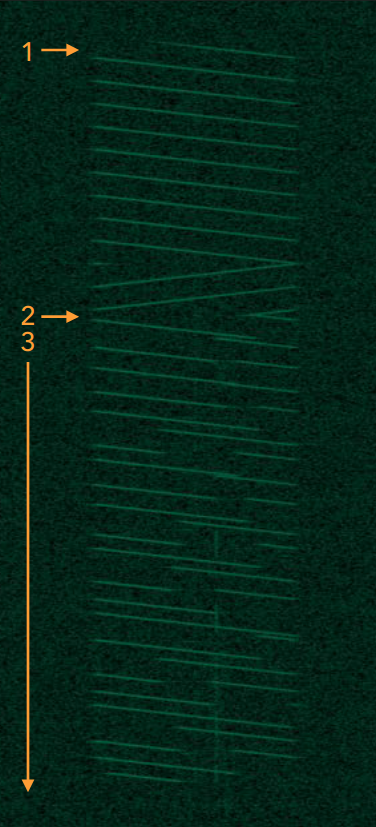
\includegraphics[width=0.8\textwidth, height=6cm]{lora_signal.png} 
        \caption{ LoRa signal}
        \label{lora1}
    \end{subfigure}
    \hspace{0.5cm}%
    \begin{subfigure}{0.7\textwidth}
        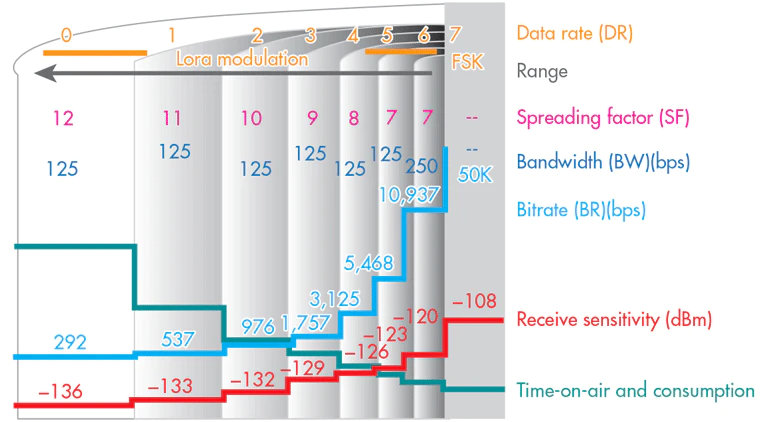
\includegraphics[width=\textwidth, height=6cm]{lora_properties.png}
        \caption{ Properties of LoRa signal}
        \label{lora2}
    \end{subfigure}
    \caption{Lora signal (left) and different properties of LoRa with their effects on range, bit rate, receiver sensitivity, time on air and consumption (right). Image sources:\cite{lora_github}\cite{lora_philly}}
    \label{lora}
\end{figure}

This kind of modulation gives LoRa extreme resiliency against interference of other radio frequency signals that might be using the same frequency band\cite{lora_article}\cite{lora_philly}.
For example, on a lower part of Figure \ref{lora1} we can see a signal with constant frequency transmitting inside bandwidth window that LoRa signal is using.
This kind of interference is easily filtered out by a LoRa receiver.

Size of a bandwidth window, rate of frequency change (also known as a spreading factor) and transmitting power further define LoRa signal.
With these factors we can influence range, power consumption and bit rate of a LoRa signal.
For example, as seen on Figure \ref{lora2}, by increasing spreading factor we increase time on air thus giving the receiver more time to sample signal, which leads to better sensitivity but increases power consumption.

While LoRa defines the physical layer, LoRaWAN defines media access control protocol for wide area networks, which are built on top of LoRa\cite{lora_article}.
Its specification is open, so any one can implement it.
LoRaWAN takes care of communication between end devices and gateways and manages communication frequency bands, data rate and transmitting power.

LoRaWAN has a star of stars topology\cite{lora_article}.
Devices deployed in the field transmit messages on frequency bands that differ from region to region. 
Messages are received by gateways which relay them to the network server.
Network server displays relayed messages, decodes them and sends them to various applications.
If the same message is heard by several gateways, the server drops all duplicates.
Server also decides which gateway will send a downlink message to a specific device. 

Because LoRaWAN operates on an unlicensed ISM band, anyone can setup up their network without any licensing fees.
For some use cases a single gateway with internet connection is enough to provide coverage to a large number of devices.


\section{ Thermal cameras}

Thermal cameras are transducers that convert infrared (IR) radiation into electrical signals, which can be used to form a thermal image.
A comparison between a normal and a thermal image can be seen on figure \ref{thermal_comparison}.
IR is an electromagnetic (EM) radiation and covers part of EM spectrum that is invisible to the human eye.
IR spectrum covers wavelengths from 780 \si{\micro\meter} to 1 \si{\milli\meter}, but only small part of that spectrum is used for IR imaging (from 0.9 \si{\micro\meter} to 14 \si{\micro\meter})\cite{thermal_book}.
We can broadly classify IR cameras into two categories: photon detectors or thermal detectors\cite{thermal_book}.
Photon detectors convert absorbed EM radiation directly into electric signals by the change of concentration of free charge carriers\cite{thermal_book}.
Thermal detectors covert absorbed EM radiation into thermal energy, raising the detector temperature\cite{thermal_book}. 
Change of detector's temperature is then converted into an electrical signal.
Since photon detectors are expensive, large and therefore unsuitable for our use case, we will not describe them in greater detail.
\newline 

\begin{figure}[ht]
    \begin{subfigure}{0.5\textwidth}
        \centering
        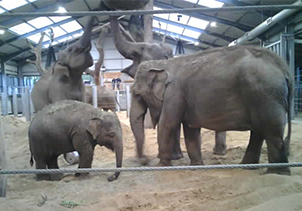
\includegraphics[width=1.0\linewidth, height=5cm]{thermal_sample_b.png} 
    \end{subfigure}
    \begin{subfigure}{0.5\textwidth}
        \centering
        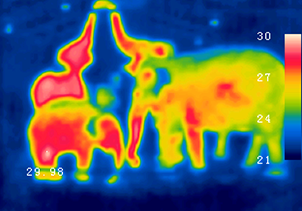
\includegraphics[width=1.0\linewidth, height=5cm]{thermal_sample_a.png}
    \end{subfigure}
    \caption{Comparison between a picture taken with a normal camera (left) and image taken with a low resolution thermal camera FLIR Lepton 2.5 (right). Image source: Arribada Initiative\cite{thermal_comparison}}
    \label{thermal_comparison}
\end{figure}

Common examples of thermal detectors are thermopiles and microbolometers. 
Thermopiles are composed of several thermocouples.
Thermocouples consists of two different metals joined at one end, which is known as hot junction.
Other two ends of the metals are known as cold junctions.
When there is a temperature difference between the hot and cold junctions, voltage proportional to that difference is generated on open ends of the metals.
To increase voltage responsivity, several thermocouples are connected in series to form a thermopile\cite{thermal_book}.
Thermopiles have lower responsivity when compared to microbolometers, but they do not require temperature stabilization\cite{thermal_book}.

Microbolometers can be found in most IR cameras today\cite{thermal_book}. 
They are sensitive to IR wavelengths of 8 to 14 \si{\micro\meter}, which is a part of longwave infrared region (LWIR)\cite{thermal_book}.
Measuring part of an microbolometer is known as focal point array (FPA) (Figure \ref{FPA}).
FPA consists of IR thermal detectors, bolometers (Figure \ref{FPA_pixel}), that convert IR radiation into electric signal.
Each bolometer consists of an absorber material connected to an readout integrated circuit (ROIC) over thermally insulated, but electrically conductive legs\cite{thermal_article}.
\newline

\begin{figure}[h]
    \begin{subfigure}{0.5\textwidth}
        \centering
        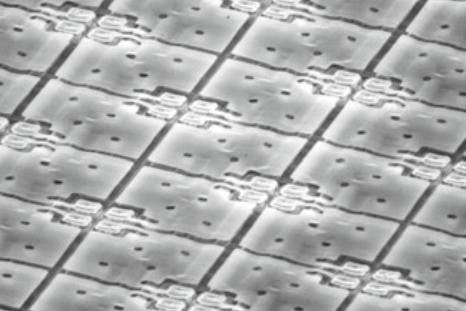
\includegraphics[width=1.0\linewidth, height=5cm]{FPA.png} 
        \caption{Focal point array}
        \label{FPA}
    \end{subfigure}
    \begin{subfigure}{0.5\textwidth}
        \centering
        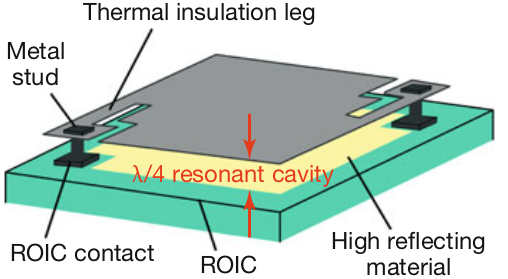
\includegraphics[width=1.0\linewidth, height=5cm]{FPA_pixel.png}
        \caption{Bolometer}
        \label{FPA_pixel}
    \end{subfigure}

    \caption{(a) Focal point array under electronic microscope. (b) Bolometer with $\lambda /4$ resonant cavity. Image source: Vollmer, Möllmann\cite{thermal_book}}
    \label{FPA_microbolo}
\end{figure}

Absorber material is made either out of metals such as gold, platinum, titanium or more commonly out of semiconductors such as vanadium-oxide (VOx)\cite{thermal_article}.
Important property of absorber materials is that electrical resistance changes proportionally with material's temperature\cite{thermal_book}.
When IR radiation hits absorber material, it is converted into thermal energy, which raises absorber's temperature, thus changing its resistance.
To detect change in resistance, ROIC applies steady-state bias current to absorber material, while measuring voltage over conductive legs\cite{thermal_book}. 

When deciding between different types of thermal cameras we are often comparing them in the terms of cost, size and image resolution.
One important property that also has to be taken into account is temperature sensitivity, also known as noise equivalent temperature difference (NETD).
NETD is measured in \si{\milli\kelvin} and tells us minimum temperature difference that can still be detected by a thermal camera.
In microbolometers NETD is proportional to the thermal conductance of absorber material, among other factors\cite{thermal_book}.
Thermal conductance of bolometers is minimized by enclosing FPA into vacuum chamber, thus excluding thermal convection and conduction due to surrounding gasses.
Only means of heat transfer that remain are radiant heat exchange (highly reflective material below absorber is minimizing its radiative losses) and conductive heat exchange through supportive legs.
NETD also depends on the temperature inside the camera, higher ambient temperatures can raise the internal temperature, thus increasing NETD and noise present in thermal image.
Today's thermopiles can achieve NETD of 100 \si{\milli\kelvin}, microbolometers 45 \si{\milli\kelvin}, while photon detectors can have NETD of 10 \si{\milli\kelvin}.
Although tens of \si{\milli\kelvin} does not seem a lot, we can see on Figure \ref{NETD} what a difference of 20 \si{\milli\kelvin} means for image resolution and noise.
\newline

\begin{figure}[ht]
    \begin{subfigure}{0.5\textwidth}
        \centering
        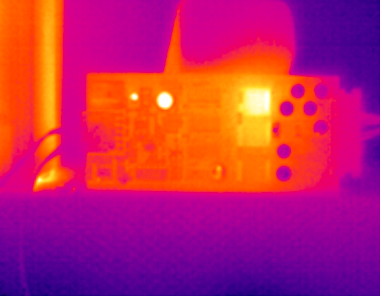
\includegraphics[width=1.0\linewidth, height=5cm]{NETD_60mk.png} 
        \caption{NETD is 60 \si{\milli\kelvin}}
        \label{NETD_60mk}
    \end{subfigure}
    \begin{subfigure}{0.5\textwidth}
        \centering
        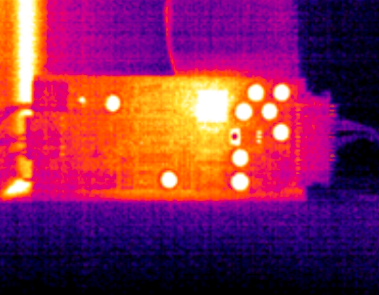
\includegraphics[width=1.0\linewidth, height=5cm]{NETD_80mk.png}
        \caption{NETD is 80 \si{\milli\kelvin}}
        \label{NETD_80mk}
    \end{subfigure}

    \caption{Comparison of images of the same object taken with cameras with different NETD values. Low NETD values are more appropriate for object recognition. Image source: MoviTherm \cite{NETD}}
    \label{NETD}
\end{figure}


\subsection{ Choosing the thermal camera}

Choice of thermal camera was made by Arribada Initiative\cite{thermal_comparison}.
They tested several different thermopiles and microbolometers, while searching for desired properties.
Camera had to be relatively inexpensive and small enough so that it could be integrated into relatively small housing.
Main property that they searched for was that elephants could be easily recognized from thermal images.
That meant that camera needed to have decent resolution and low NETD.
Cameras were tested in Whipsnade Zoo and the Yorkshire Wildlife Park where images of elephants and polar bears could be made.

They tested two thermopile cameras (Heimann 80x64, MELEXIS MLX90640) and two microbolometer cameras (ULIS Micro80 Gen2, FLIR Lepton 2.5).
Although thermopile cameras were cheaper from microbolometer cameras, quality of images they produced was inferior, as can be seen on Figure \ref{thermal_comparison_images}.

\begin{figure}[ht]
    \begin{subfigure}{0.5\textwidth}
        \centering
        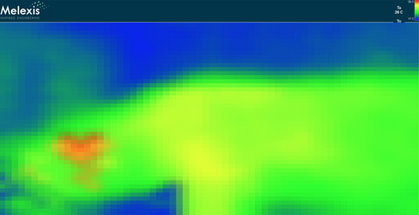
\includegraphics[width=1.0\linewidth, height=4.5cm]{thermal_comparison_a.png} 
        \label{thermal_comparison_a}
    \end{subfigure}
    \begin{subfigure}{0.5\textwidth}
        \centering
        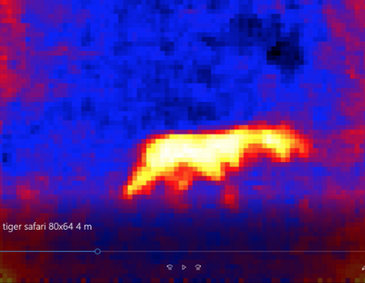
\includegraphics[width=1.0\linewidth, height=4.5cm]{thermal_comparison_b.png} 
        \label{thermal_comparison_b}
    \end{subfigure}
    \begin{subfigure}{0.5\textwidth}
        \centering
        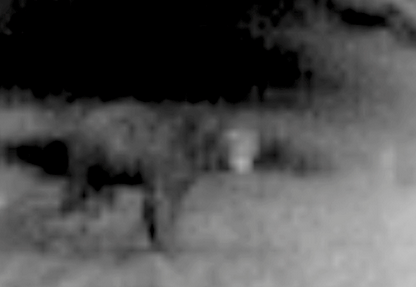
\includegraphics[width=1.0\linewidth, height=4.5cm]{thermal_comparison_c.png} 
        \label{thermal_comparison_c}
    \end{subfigure}
    \begin{subfigure}{0.5\textwidth}
        \centering
        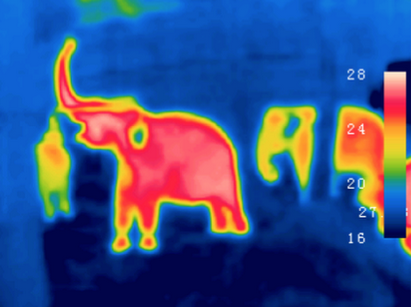
\includegraphics[width=1.0\linewidth, height=4.5cm]{thermal_comparison_d.png} 
        \label{thermal_comparison_d}
    \end{subfigure}
\caption[Comparison of image quality made by different thermal cameras]{, MELEXIS MLX90640 (top left), Heimann 80x64 (top right), ULIS Micro80 Gen2 (bottom left) and FLIR Lepton 2.5 (bottom right). Image source: Arribada Initiative \cite{thermal_comparison}}
    \label{thermal_comparison_images}
\end{figure}

MELEXIS MLX90640 camera had resolution of 32 x 24 pixels and NETD of 100 \si{\milli\kelvin}, while Heimann camera had resolution of 80 x 64 pixels and NETD of 400 \si{\milli\kelvin}.
It was concluded that images taken by either one of thermopile cameras could not be used for object recognition, merely only if object was present or not\cite{thermal_comparison}.

Microbolometers produced better results.
Both Ulis Micro80 and FLIR Lepton had similar resolution, 80 x 80 and 80 x 60 respectively, but Ulis Micro80 had two times bigger NETD compared to FLIR Lepton camera, 100 \si{\milli\kelvin} and 50 \si{\milli\kelvin}, respectively.
Images produced by FLIR Lepton were much cleaner, so it was chosen as appropriate camera for the task.

It is important to note that FLIR Lepton, as all microbolometers, requires frequent calibration to function properly.
In temperature non-stabilized cameras small temperature drifts can have a major impact on image quality\cite{thermal_book}.
Calibration is done either by internal algorithms of the camera or by exposing the camera to uniform thermal scene.
FLIR Lepton camera comes with a shutter, which acts as a uniform thermal signal and enables regular calibration.
Calibration in FLIR Lepton is by default automatic, triggering at startup and every 3 minutes afterwards or if camera temperature drifts for more than 1.5 \si{\celsius}.

%%
%\chapter{ Neural Network model design}
%In this chapter we will describe the design of neural network that will be able to process thermal images and decide what object they contain.
Workflow that we will follow will largely be a combination of workflows presented in Figures \ref{ml_workflow} and \ref{micro_workflow}.

We will first set concrete objectives, which will dictate what exactly we want to accomplish, while keeping in consideration various constraints.
We will then explore the dataset provided by Arribada Initiative, analyze different class representations and decide if it is appropriate for accomplishing objectives that we set earlier.

After dataset exploration we had to setup our development environment.
As software for creating and training ML models consists of many components and dependencies it is important to start with something that we know it works.
We will describe our AWS server setup, how we moved image data on it and why we decided to use Python Notebooks for algorithm development.

Image preparation was important step before model creation, as wanted to keep track of various metadata labels that were assigned to each image.
This involved parsing a large excel table and connecting images with correct labels.
Image preprocessing such as mean normalization and augmentation was then done.
We then designed and trained few CNN models with varying complexities and observed how well they behave on thermal image dataset.
We then optimized models with TFLite tools and compared accuracies and model sizes.
Models were then converted into a C char array format, ready to be tested on a actual microcontroller.

We will finish this chapter by describing the same workflow, but by using tools that Edge Impulse provides to the point where we will have our model ready to run on a microcontroller.
Using Edge Impulse will generally require less knowledge, less time and will lead to better results when compared to our setup.


\section{ Objectives}

The accuracy of our early detection system should be equal or similar to the one of human observer, no matter if we are operating in the daytime or nighttime.
Although our system will be placed on the paths that are regularly traversed by elephants, this does not mean that they will be only possible object on a image taken by a thermal camera.
Humans and various livestock, such as goats and cows, could also be photographed.
This means that we want to avoid reporting false positives, which means that our system should not incorrectly label a human or a livestock animal as an elephant.
At the same time we want avoid false negatives, where an elephant could pass by our system undetected.
These kind of mistakes could undermine the community's confidence of our early detection system and defeat our purpose.
This means that besides elephant detection, we should also focus on correctly labeling humans and livestock, while also providing a nature/random class for all other unexpected objects or simply images of nature.

It would be beneficial if thermal camera can take several pictures of the same object, thus increasing the confidence of computed label of the object.
However this is constrained by the image processing time and camera's field of view.
Thermal camera FLIR Lepton has a horizontal field of view of 57 degrees.
The closer elephant passes by the thermal camera the quicker he will traverse the camera's field of view, thus giving the camera less time for capture.
This problem can be solved by optimizing the execution time of the ML model or by placing the early detection system on far enough position from expected elephant's path.
As latter option might not be always possible, we should strive to keep the whole image processing time as short as possible.

Finally, as our neural network will be deployed on a microcontroller and not on a computer or a server we have to keep it simple and small.
Extra model complexity that might bring us few percents of accuracy will not matter much, if our model would be too large to fit on a microcontroller or too slow to run.


To summarize:
\begin{itemize}
    \item We will create an image classification ML model that will be capable of processing a thermal image and sorting it into one of possible 4 categories: elephant, human, cows and nature/random.
    \item Total image processing time should be as short as possible, we should try to keep it under 2 seconds.
    \item Model should be small enough to fit on a microcontroller of our choice, while still leaving some space for application code. Microcontroller of our choice (STM32F767) has 2 MB of flash memory so model size should be smaller than that.
\end{itemize}


\section{ Exploring the dataset}
Show images, 
how and by who were they made, 
what was their original purpose
show ratios of different meta data
what is missing from dataset
Describe how you made missing pictures
make a picture of a setup

\section{ Development enviroment }
Linux server on AWS with Tensorflow preinstalled
Python Notebooks
How and why did you chose this setup
\section{ Image preparation}

\section{ Model creation and training (Rethink title)}
train few different models
with different accuracies

\section{ Optimising models}
Comparison between different sizes and accuracies

\section{ Edge Impulse (SHOULD this be here like that, how should i go about this)}

%
%\chapter{ Planning and design of early warning system}
%\lipsum



\chapter{ Measurements and results}
\section{ Comparison of models}\label{model_comparisons}

As mentioned in Section \ref{cnn_ref}, we used Keras Tuner model to find hyperparameters that would yield the highest accuracy.
Instead of hard-coding hyperparameters when building a model with Keras API, we defined a search space of possible values with \verb|HyperParameter| class and used that as a hyperparameter.

We passed the created model to a \verb|RandomSearch| class, with few other parameters such as batch size, number of epochs and maximum number of trials.
As we started the hyperparameter search, Keras Tuner started picking a randomly set of hyperparameters, which were used to train a model.
This process was repeated for a trial number of times.
Used hyperparameters and achieved accuracy on the validation set for each trained model were logged in a text file for later use.

After training several different models we picked a few and compared them.
Comparison of models trained in Edge Impulse Studio was also done.

To distinguish models from one another we decided to mark them with a number and letters \textit{a}, \textit{b}, \textit{ei} and \textit{tl}.
Models with letters \textit{a} and \textit{b} were trained using our system.
Models marked with \textit{ei} and \textit{tl} were in Edge Impulse Studio, former with a setup comparable to the ours, latter with Transfer Learning technique.
Tables that are shown below list one of the metrics as accuracy.
With accuracy we mean validation accuracy, it tells us how well model performed on a validation dataset.

\subsection{ Hyperparameter search space and results analysis}

General structure of CNN model was already described in Section \ref{cnn_ref} and in Figure \ref{model_code}.
We decided to search for the following hyperparameters: 

\begin{itemize}
    \item Number of filters in all three convolutional layers (can be different for each layer)
    \item Size of filters in all three convolutional layers (same for all layers)
    \item Size of the dense layer
    \item Dropout rate 
    \item Learning rate
\end{itemize}

Possible values of hyperparameters (also known as hyperparameter search space) are specified in Table \ref{hyper_table1}.
\newline
\begin{table}[ht]
    \centering
    \caption{ First hyperparameter search space}
    \rowcolors{2}{white}{gray!25}
    \begin{tabular}{@{} *5l @{}}    \toprule
        \textbf{Hyperparameter} & \textbf{Set of values}\\\midrule
        \verb|FilterNum1|       & From 16 to 80, with a step of 8\\ 
        \verb|FilterNum2|       & From 16 to 80, with a step of 8\\ 
        \verb|FilterNum3|       & From 16 to 80, with a step of 8\\
        \verb|FilterSize|       & 3 x 3 or 3 x 4\\
        \verb|DenseSize|        & From 16 to 96, with a step of 8\\
        \verb|DropoutRate|      & From 0.2 to 0.5, with a step of 0.05\\
        \verb|LearningRate|     & 0.0001 or 0.0003\\\toprule
        \textbf{Random search}  & \textbf{value}\\
        \textbf{variable}       & \\\midrule
        \verb|EPOCHS|           & 25\\
        \verb|BATCH_SIZE|       & 100\\
        \verb|MAX_TRIALS|       & 300\\\bottomrule
    \end{tabular}
    \label{hyper_table1}
\end{table}

Search space of \verb|FilterNumX|, \verb|DenseSize| and \verb|DropoutRate| hyperparameters were chosen based on initial training tests conducted on a thermal image dataset and other various models that were trained on similar data.
Value of \verb|FilterSize| is usually 3 x 3, however, most of example ML projects that we could find on the Internet were training on image data of the same dimensions.
We wanted to test how would a filter with the same ratio of dimensions as image data (3 x 4 and 60 x 80 respectively) perform.
Hyperparameter \verb|learning_rate| was chosen heuristically, we saw that 10 times higher values, such as 0.001 or 0.003, would leave model's accuracy stuck at suboptimal optima, from where it could not be improved anymore.

We also had to set 3 variables that directly affected how long will random search last.
From initial tests we saw that models usually reached maximum possible accuracy around \nth{20} epoch, to give some headroom we set the number of epochs to 25.
We kept batch size relatively small, at 100, which meant that weights would get updated regularly.
Hyperparameter \verb|MAX_TRIALS| had the biggest impact on the training time, we set it to 300.

The training lasted for about 12 hours. 
After it was done we compiled a list of all 300 trained models and their different hyperparameter values, number of parameters and achieved accuracies.
Part of it can be seen in Table \ref{hyper_results1}.

After analysing results we came to several conclusions:

\begin{enumerate}
    \item We saw that almost all trained models, except for the last one, achieved accuracy above 90 \%. This proved that the general architecture of the model was appropriate for the problem.
    \item We could not see any visible correlation between a specific choice of a certain hyperparameter and accuracy. This showed that selection of hyperparameters is a non-heuristic task, at least for our particular problem.
    \item Filter of size 3 x 4 did not perform significantly better compared to one with size 3 x 3. 
    \item First 200 models cover an accuracy range of 0.62 \%. However inside of this range number of parameters varies hugely, for example, the model \textit{192a} has more than 8 times fewer parameters than the model \textit{96a}, although the difference in accuracy (0.27 \%) is negligible.
\newline
\end{enumerate}
\begin{table}[ht]
    \centering
    \caption{ Partial results of first random search of hyperparameters}
    \rowcolors{2}{gray!25}{white}
    \begin{tabular}{llllllllrl}
    \textbf{Model ID} & \rot{FilterNum1} & \rot{FilterNum2} & \rot{FilterNum3} & \rot{DenseSize} & \rot{DropoutRate}  &\rot{FilterSize} & \rot{LearningRate} & \rotatebox{45}{\parbox{2cm}{Number of parameters}} & \rot{Accuracy[\%]}  \\\toprule
        0a & 72 & 80 & 64 & 72 & 0.4  & 3x4 & 0.0003 & 1,514,400 & 98.35\\
        1a & 32 & 40 & 72 & 56 & 0.35 & 3x4 & 0.0001 & 1,260,332 & 98.31\\
        2a & 40 & 48 & 32 & 64 & 0.35 & 3x4 & 0.0001 &   656,797 & 98.31\\
        3a & 56 & 16 & 48 & 72 & 0.4  & 3x4 & 0.0001 & 1,057,924 & 98.28\\
        4a & 80 & 64 & 40 & 96 & 0.45 & 3x4 & 0.0003 & 1,245,788 & 98.28\\\midrule
       96a & 16 & 32 & 72 & 80 & 0.25 & 3x4 & 0.0001 & 1,762,508 & 98.00\\
       97a & 72 & 56 & 40 & 56 & 0.45 & 3x4 & 0.0003 &   748,580 & 98.00\\
       98a & 32 & 24 & 24 & 48 & 0.35 & 3x3 & 0.0001 &   358,308 & 98.00\\
       99a & 48 & 16 & 40 & 40 & 0.45 & 3x3 & 0.0003 &   493,412 & 98.00\\
      100a & 24 & 72 & 64 & 40 & 0.45 & 3x3 & 0.0003 &   844,684 & 98.00\\\midrule
      191a & 64 & 56 & 16 & 52 & 0.4  & 3x3 & 0.0001 &   386,996 & 97.76\\
      192a & 48 & 40 & 24 & 24 & 0.4  & 3x4 & 0.0001 &   208,172 & 97.73\\
      193a & 56 & 64 & 72 & 24 & 0.25 & 3x4 & 0.0003 &   617,692 & 97.73\\
      194a & 48 & 72 & 48 & 32 & 0.25 & 3x4 & 0.0003 &   544,652 & 97.73\\\midrule
      295a & 48 & 32 & 64 & 16 & 0.5  & 3x4 & 0.0001 &   351,012 & 95.87\\
      296a & 40 & 24 & 56 & 24 & 0.5  & 3x4 & 0.0001 &   431,572 & 95.77\\
      297a & 56 & 16 & 80 & 16 & 0.2  & 3x4 & 0.0001 &   411,020 & 95.63\\
      298a & 24 & 16 & 48 & 24 & 0.5  & 3x4 & 0.0001 &   359,924 & 94.46\\
      299a & 40 & 48 & 56 & 16 & 0.35 & 3x3 & 0.0003 &   310,860 & 82.86\\\bottomrule
    \end{tabular}
    \label{hyper_results1}
\end{table}
It was apparent from results that large models are not necessary to achieve high accuracy on our training data, so we decided to run the random search of hyperparameters again.
This time we lowered the maximum and the minimum numbers of filters and size of the dense layer.
We decreased all steps from 8 to 2, thus increasing the number of possible configurations.
We decided to lower the bottom boundary of \verb|DropoutRate| from 0.2 to 0.0, which means that some models will not be using dropout layer at all.
We expected that training without dropout layer would produce suboptimal results, however, we wanted to test it.
Redefined search space for second random search can be seen in Table \ref{hyper_table2}
We increased the number of \verb|MAX_TRIALS| from 300 to 500, as we were expecting that more models will end up underfitting and also because there would be more possible options because of smaller step size.
Partial table of results of random hyperparameter search can be seen in Table \ref{hyper_results2}.

\begin{table}[ht]
    \centering
    \caption{ Second hyperparameter search space}
    \rowcolors{2}{white}{gray!25}
    \begin{tabular}{@{} *5l @{}}    \toprule
        \textbf{Hyperparameter} & \textbf{Set of values}\\\midrule
        \verb|FilterNum1|       & From 4 to 48, with a step of 2\\ 
        \verb|FilterNum2|       & From 4 to 48, with a step of 2\\ 
        \verb|FilterNum3|       & From 4 to 48, with a step of 2\\
        \verb|FilterSize|       & 3 x 3 or 3 x 4\\
        \verb|DenseSize|        & From 4 to 48, with a step of 2\\
        \verb|DropoutRate|      & From 0.0 to 0.5, with a step of 0.05\\
        \verb|LearningRate|     & 0.0001 or 0.0003\\\toprule
        \textbf{Random search}  & \textbf{value}\\
        \textbf{variable}       & \\\midrule
        \verb|EPOCHS|           & 25\\
        \verb|BATCH_SIZE|       & 100\\
        \verb|MAX_TRIALS|       & 500\\\bottomrule
    \end{tabular}
    \label{hyper_table2}
\end{table}

\begin{table}[ht]
    \centering
    \caption{ Partial results of second random search of hyperparameters}
    \rowcolors{2}{gray!25}{white}
    \begin{tabular}{llllllllrl}
    \textbf{Model ID} & \rot{FilterNum1} & \rot{FilterNum2} & \rot{FilterNum3} & \rot{DenseSize} & \rot{DropoutRate}  &\rot{FilterSize} & \rot{LearningRate} & \rotatebox{45}{\parbox{2cm}{Number of parameters}} & \rot{Accuracy[\%]}  \\\toprule
        0b & 40 & 20 & 20 & 48 & 0.25 & 3x4 & 0.0001 & 304,216 & 98.14\\
        1b & 44 & 10 & 28 & 42 & 0.2  & 3x4 & 0.0003 & 362,264 & 98.14\\
        2b & 18 & 38 & 26 & 38 & 0.1  & 3x4 & 0.0003 & 316,956 & 98.11\\\midrule
       95b & 20 & 16 & 34 & 40 & 0.3  & 3x3 & 0.0003 & 416,230 & 97.62\\
       96b & 46 & 42 & 28 & 32 & 0.4  & 3x3 & 0.0003 & 297,466 & 97.62\\
       97b & 30 & 26 & 30 & 34 & 0.2  & 3x3 & 0.0001 & 320,570 & 97.59\\\midrule
      195b & 28 & 16 & 40 & 24 & 0.1  & 3x3 & 0.0001 & 298,252 & 97.31\\
      196b & 44 & 30 & 32 & 20 & 0.3  & 3x4 & 0.0003 & 220,098 & 97.31\\
      197b & 46 & 40 & 10 & 40 & 0.1  & 3x3 & 0.0001 & 140,874 & 97.31\\\midrule
      295b & 20 &  8 & 34 & 26 & 0.3  & 3x3 & 0.0003 & 269,464 & 96.90\\
      296b & 18 & 16 & 10 & 20 & 0.3  & 3x4 & 0.0003 &  65,740 & 96.87\\
      297b &  8 & 22 & 28 & 16 & 0.1  & 3x3 & 0.0001 & 141,742 & 96.87\\\midrule
      395b & 10 & 20 & 12 & 30 & 0.0  & 3x3 & 0.0001 & 112,246 & 96.87\\
      396b & 24 & 24 & 46 & 18 & 0.2  & 3x3 & 0.0003 & 263,924 & 96.14\\
      397b &  6 & 18 & 12 & 24 & 0.4  & 3x4 & 0.0001 &  90,520 & 96.11\\\midrule
      497b & 42 & 30 & 22 &  6 & 0.4  & 3x3 & 0.0003 &  57,386 & 82.86\\
      498b &  4 &  4 & 20 & 12 & 0.4  & 3x3 & 0.0003 &  72,992 & 82.86\\
      499b & 32 & 36 & 36 &  4 & 0.15 & 3x3 & 0.0001 &  65,648 & 82.86\\\bottomrule
    \end{tabular}
    \label{hyper_results2}
\end{table}

\clearpage
Some observations:
\begin{enumerate}
    \item We can see that the accuracy of the best model \textit{0b} compared to the best model \textit{0a} from the previous search is only 0.21 \% lower, although it has about 5 times fewer parameters.
    \item Although that it might seem that \verb|FilterSize| of 3 x 4 yields best results, we did not saw a strong tendency towards 3 x 3 or 3 x 4 filter size after manually analyzing best 30 models.
    \item We can see that the worst three models have the same accuracy of 82.86 \%, same as the worst-performing model from the first random search. There are 82.86 \% images of elephants in the validation class, which means that the model probably assigned all validation images to elephant class and was satisfied with achieved accuracy.
    \item We can see that the model \textit{296b} has a quite low number of parameters, only 65,740 when compared to its neighbours.
\end{enumerate}

\subsection{ Comparison of selected, re-trained models}
    
Two random searches gave us a large number of different models to choose from.
In every other ML application where the execution time would not be a constraint, we could simply take the best performing model and be done with it.
In our case, we had to make a trade-off between model's accuracy and execution speed.

For comparison and later on device performance testing we decided to pick and retrain\footnotemark 6 models: \textit{0a}, \textit{2a}, \textit{0b}, \textit{172b}, \textit{338b} and \textit{460b}, their properties are listed in Table \ref{hyper_selection}.

Chosen models vary greatly in the number of parameters.
Models \textit{0a}, \textit{2a}, \textit{0b} have high number of parameters but their accuracy is high.
Models \textit{172b}, \textit{338b} and \textit{460b} were chosen because of their small size and reasonably good accuracy.
\footnotetext{Retraining was required as Keras Tuner module only saved hyperparameter settings during search and not each trained model.
As the weights are initially randomized, the accuracy of retrained models is going to be similar but not exact when compared to the accuracy returned by the random search.}

\begin{table}[ht]
    \centering
    \caption{ Properties of selected models}
    \rowcolors{2}{gray!25}{white}
    \begin{tabular}{llllllllrl}
    \textbf{Model ID} & \rot{FilterNum1} & \rot{FilterNum2} & \rot{FilterNum3} & \rot{DenseSize} & \rot{DropoutRate}  &\rot{FilterSize} & \rot{LearningRate} & \rotatebox{45}{\parbox{2cm}{Number of parameters}} & \rot{Accuracy[\%]}  \\\toprule
        0a & 72 & 80 & 64 & 72 & 0.4  & 3x4 & 0.0003 & 1,514,400 & 98.35\\
        2a & 40 & 48 & 32 & 64 & 0.35 & 3x4 & 0.0001 &   656,797 & 98.31\\
        0b & 40 & 20 & 20 & 48 & 0.25 & 3x4 & 0.0001 &   304,216 & 98.14\\
      172b & 42 & 44 &  8 & 14 & 0.1  & 3x4 & 0.0001 &    60,672 & 97.38\\
      338b &  4 & 18 &  6 & 10 & 0.05 & 3x4 & 0.0003 &    20,290 & 96.63\\
      460b &  6 & 28 &  4 &  8 & 0.1  & 3x4 & 0.0003 &    13,114 & 93.60\\\bottomrule
    \end{tabular}
    \label{hyper_selection}
\end{table}

As we are dealing with an imbalanced dataset, where 82.86 \% of our validation data consists of elephant images, accuracy is not the best metric to use when comparing models.
Simply classifying all images into elephant class would yield an accuracy of 82.86 \%, which sounds high, although it would not actually do any classification.

When analysing the performance of a model on an imbalanced dataset it is more appropriate to use precision and recall metrics\footnotemark.
They can give us a better idea of how well the model is performing on data of specific classes.
Calculated metrics can be seen in Table \ref{precision_recall_table}, we abbreviated precision to P and recall to R for clarity.
We also colour coded each table row, bright green shows the highest value in the row, red shows the lowest, light-green and orange colours show values in between.
\footnotetext{Precision tells us what percentage of data points in a specific predicted class fall into that class.
Recall tells us what percentage of data points inside a certain class were actually predicted correctly\cite{geron}.}
\begin{table}[ht]
    \caption{ Precision and recall metrics of trained models}
    \rowcolors{2}{gray!25}{white}
    \makebox[\textwidth]{%
    \begin{tabular}{lrrrrrrrrr}\toprule
        \textbf{Model ID}                 & 0a & 2a & 0b & 172b & 338b & 460b\\\toprule
        \textbf{Metrics}                &&&&&\\\toprule
        accuracy[\%]                    & \cellcolor{tbgreen} 98.18     
                                        & \cellcolor{tbgreeny}98.04   
                                        & \cellcolor{tbgreeny}98.04   
                                        & \cellcolor{tbyellow}96.80  
                                        & \cellcolor{tbyellow}96.28  
                                        & \cellcolor{tbred}   93.4 \\

        Number of parameters            & \cellcolor{tbred}  1,515K 
                                        & \cellcolor{tbyellow} 657K 
                                        & \cellcolor{tbyellow} 304K 
                                        & \cellcolor{tbyellow}  61K 
                                        & \cellcolor{tbgreeny}  20K 
                                        & \cellcolor{tbgreen}   13K\\\midrule

        P of elephant class[\%]         & \cellcolor{tbyellow}99.22     
                                        & \cellcolor{tbgreen}99.46   
                                        & \cellcolor{tbyellow}99.25   
                                        & \cellcolor{tbgreeny}99.29  
                                        & \cellcolor{tbyellow}98.80  
                                        & \cellcolor{tbred}97.80\\
        P of human class[\%]            & \cellcolor{tbgreen}96.92     
                                        & \cellcolor{tbgreeny}95.38   
                                        & \cellcolor{tbgreeny}95.38   
                                        & \cellcolor{tbyellow}92.00  
                                        & \cellcolor{tbyellow}91.69  
                                        & \cellcolor{tbred}80.31\\
        P of cow class[\%]              & \cellcolor{tbgreeny}90.99     
                                        & \cellcolor{tbgreen}93.69   
                                        & \cellcolor{tbyellow}90.09   
                                        & \cellcolor{tbyellow}84.68  
                                        & \cellcolor{tbyellow}75.68  
                                        & \cellcolor{tbred}69.37\\
        P of nature/random class[\%]    & \cellcolor{tbgreeny}77.42     
                                        & \cellcolor{tbyellow}64.52   
                                        & \cellcolor{tbgreen}79.03   
                                        & \cellcolor{tbyellow}46.77  
                                        & \cellcolor{tbyellow}59.68 
                                        & \cellcolor{tbred}40.32\\\midrule
        R of elephant class[\%]         & \cellcolor{tbgreen}99.29     
                                        & \cellcolor{tbyellow}98.80   
                                        & \cellcolor{tbgreeny}98.84   
                                        & \cellcolor{tbyellow}97.87  
                                        & \cellcolor{tbyellow}98.43  
                                        & \cellcolor{tbred}97.39\\
        R of human class[\%]            & \cellcolor{tbyellow}93.20     
                                        & \cellcolor{tbgreeny}94.51   
                                        & \cellcolor{tbgreen}95.09   
                                        & \cellcolor{tbyellow}91.44  
                                        & \cellcolor{tbyellow}89.22  
                                        & \cellcolor{tbred}85.57\\
        R of cow class[\%]              & \cellcolor{tbgreeny}94.39     
                                        & \cellcolor{tbyellow}92.04   
                                        & \cellcolor{tbgreen}96.15   
                                        & \cellcolor{tbyellow}89.52  
                                        & \cellcolor{tbyellow}84.00  
                                        & \cellcolor{tbred}81.91\\
        R of nature/random class[\%]    & \cellcolor{tbyellow}87.27     
                                        & \cellcolor{tbgreen}97.56   
                                        & \cellcolor{tbyellow}84.48   
                                        & \cellcolor{tbgreeny}93.55  
                                        & \cellcolor{tbyellow}67.27  
                                        & \cellcolor{tbred}28.09\\\bottomrule
    \end{tabular}}
    \label{precision_recall_table}
\end{table}

As we can see all six models are generally classifying elephants correctly, both precision and recall of elephant class are high, above 97 \%, which is important.
Precision and recall values of other classes are generally lower, especially for nature/random.
We can see that top three models \textit{0a}, \textit{2a} and \textit{0b} are quite similar in terms of precision and recall, which means that we can easily prefer \textit{0b}, without sacrificing accuracy. 
Models \textit{172b} and \textit{338b} perform a bit worse when compared to top three models, however, they have a low number of parameters which should translate to lower inference time.
Last model, \textit{460b}, performs the worst and it should generally not be used.

Another way to compare models performance is to look at a confusion matrix.
Figure \ref{double_cm} shows comparison between confusion matrices of \textit{0a} model on the left and \textit{460b} model on the right.
In the case of \textit{0a}, 19 elephant images were not classified correctly, and 17 images were wrongly classified as elephants.
This is not ideal, however is much better compared to performance of \textit{460b}, where 53 elephants were wrongly classified and 63 of images classified as elephants were not actually elephants.
\newline
\begin{figure}[ht]
    \begin{subfigure}{0.5\textwidth}
        \centering
        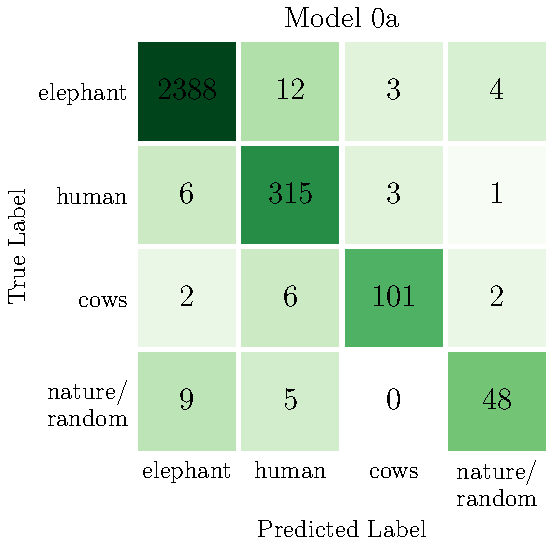
\includegraphics[width=1\linewidth]{0a_cm.pdf} 
    \end{subfigure}
    \begin{subfigure}{0.5\textwidth}
        \centering
        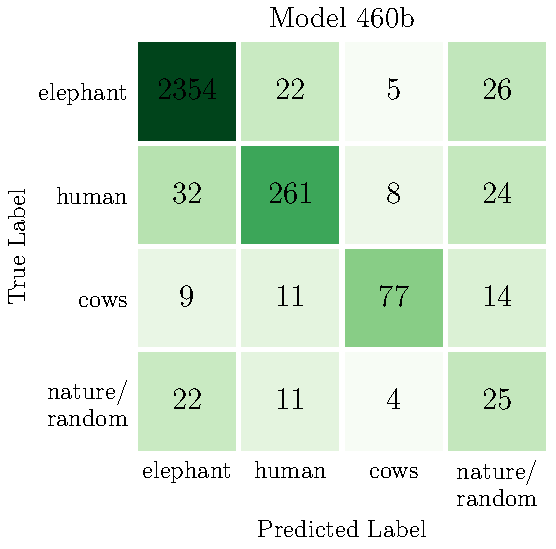
\includegraphics[width=1\linewidth]{460b_cm.pdf}
    \end{subfigure}
    \caption{Confusion matrices of \textit{0a} model (left) and \textit{460b} model (right).}
    \label{double_cm}
\end{figure}
\clearpage

\subsection{ Comparison of Edge Impulse models}

We wanted to take our 6 models and compare them against 6 Edge Impulse models that were created by using the same hyperparameters.
However, at the time of writing Edge Impulse supported only model training on images of the same dimensions.
Images with different dimensions could either be cropped or scaled to fit 1:1 ratio.
Using the same hyperparameters in Edge Impulse Studio, that were used in our models, would always create a model with a smaller number of parameters.
The smaller image creates a smaller network when compared to a bigger image, given that the rest of architecture does not change.
That meant that we could not make a direct comparison between our models and models trained in Edge Impulse Studio.
We also could not perform a random search of hyperparameters in Edge Impulse Studio, as this feature was not fully supported at the time of writing this thesis.

We decided to train a few differently sized models, using the same general CNN architecture as before, but with some minor changes in hyperparameter values.
We also trained a few models with Transfer Learning technique.
Edge Impulse offers scaled-down versions of pre-trained MobileNetV2\footnotemark NN architecture, which we used.

Tables \ref{ei_models1} and \ref{ei_models2} show properties of Edge Impulse models using CNN architecture and Transfer Learning technique, respectively. 
Table \ref{precision_recall_table_ei} shows calculated precision and recall values of Edge Impulse models using both approaches.
\footnotetext{MobileNetV2 is a efficient, lightweight NN architecture, designed for image recognition tasks, suitable for mobile applications\cite{geron}. MobileNetV2 contains width multiplier hyperparameter, which scales up or down the total number of parameters, thus providing a trade-off between accuracy and computation complexity. Edge Impulse offers three different width multiplier options: 0.35, 0.1 and 0.05.}

We used only two different versions of MobileNetV2, 0.35, and 0.1, as we saw an accuracy drop in the reduction of width multiplier hyperparameter.
In all cases the pre-trained model was followed by a one or two dense layers, with dropout layers in between.
\clearpage
\begin{table}[!htbp]
    \centering
    \caption{ Properties of Edge Impulse models using CNN architecture.}
    \rowcolors{2}{gray!25}{white}
    \makebox[\textwidth]{%
    \begin{tabular}{llllllllrl}
    \textbf{Model ID} & \rot{FilterNum1} & \rot{FilterNum2} & \rot{FilterNum3} & \rot{DenseSize} & \rot{DropoutRate}  &\rot{FilterSize} & \rot{LearningRate} & \rotatebox{45}{\parbox{2cm}{Number of parameters}} & \rot{Accuracy[\%]}  \\\toprule
        0ei & 72 & 80 & 64 & 72 & 0.4  & 3x4 & 0.0003 & 1,168,804 & 97.7\\
        1ei & 40 & 48 & 32 & 64 & 0.35 & 3x4 & 0.0001 &   503,196 & 97.5\\
        2ei & 40 & 20 & 20 & 48 & 0.25 & 3x4 & 0.0001 &   231,204 & 97.3\\
        3ei & 42 & 44 &  8 & 14 & 0.1  & 3x4 & 0.0003 &    52,272 & 96.6\\\bottomrule
    \end{tabular}}
    \label{ei_models1}
\end{table}
\bigskip
\bigskip
\bigskip
\begin{table}[!htbp]
    \centering
    \caption{ Properties of Edge Impulse models using Transfer Learning technique}
    \rowcolors{2}{gray!25}{white}
    \makebox[\textwidth]{%
    \begin{tabular}{llllllll}
        \textbf{Model ID} & \rotatebox{45}{\parbox{1cm}{Width \\Multiplier}} & \rot{DenseSize1} & \rot{DenseSize2} & \rot{DropoutRate} & \rot{LearningRate} & \rotatebox{45}{\parbox{2cm}{Number of\\parameters}} & \rot{Accuracy[\%]}  \\\toprule
        0tl & 0.35 & 16 & N/A& 0.1 & 0.0005 & 430,676 & 98.5\\
        1tl & 0.35 & 16 & 16 & 0.1 & 0.0005 & 430,948 & 98.4\\
        2tl & 0.35 & 32 & 32 & 0.1 & 0.0005 & 452,484 & 98.7\\
        3tl & 0.1  & 32 & 32 & 0.1 & 0.0005 & 135,732 & 95.7\\\bottomrule
    \end{tabular}}
    \label{ei_models2}
\end{table}
\bigskip
\bigskip
\bigskip
\begin{table}[!htbp]
    \caption{ Precision and recall metrics of trained Edge Impulse models}
    \rowcolors{2}{gray!25}{white}
    \makebox[\textwidth]{%
    \begin{tabular}{lrrrrrrrr}\toprule
        \textbf{Model ID}               & 0e    & 1e & 2e & 3e & 0tl & 1tl & 2tl & 3tl\\\toprule
        \textbf{Metrics}                &&&&&&&&\\\toprule
        Accuracy[\%]                    & \cellcolor{tbyellow} 97.7  
                                        & \cellcolor{tbyellow} 97.5  
                                        & \cellcolor{tbyellow} 97.3  
                                        & \cellcolor{tbyellow} 96.6  
                                        & \cellcolor{tbgreeny} 98.5  
                                        & \cellcolor{tbgreeny} 98.4  
                                        & \cellcolor{tbgreen} 98.7  
                                        & \cellcolor{tbred} 95.7  \\
        Number of parameters            & \cellcolor{tbred} 1,169K 
                                        & \cellcolor{tbyellow} 503K 
                                        & \cellcolor{tbgreeny} 231K 
                                        & \cellcolor{tbgreen} 52K 
                                        & \cellcolor{tbyellow} 430K 
                                        & \cellcolor{tbyellow} 431K 
                                        & \cellcolor{tbyellow} 452K 
                                        & \cellcolor{tbgreeny} 136K\\\midrule
        P of elephant class[\%]         & \cellcolor{tbgreen}  99.69 
                                        & \cellcolor{tbgreeny} 99.53 
                                        & \cellcolor{tbgreeny} 99.42 
                                        & \cellcolor{tbyellow} 99.27 
                                        & \cellcolor{tbyellow} 99.27 
                                        & \cellcolor{tbgreeny} 99.42 
                                        & \cellcolor{tbgreeny} 99.48
                                        & \cellcolor{tbred}    98.65 \\
        P of human class[\%]            & \cellcolor{tbyellow} 95.05 
                                        & \cellcolor{tbyellow} 95.05 
                                        & \cellcolor{tbyellow} 91.87 
                                        & \cellcolor{tbyellow} 91.52 
                                        & \cellcolor{tbgreen}  97.17 
                                        & \cellcolor{tbyellow} 95.41 
                                        & \cellcolor{tbgreeny} 96.47
                                        & \cellcolor{tbred}    85.16 \\
        P of cow class[\%]              & \cellcolor{tbyellow} 82.22 
                                        & \cellcolor{tbyellow} 78.89 
                                        & \cellcolor{tbyellow} 82.22 
                                        & \cellcolor{tbyellow} 79.57 
                                        & \cellcolor{tbgreen}  92.22 
                                        & \cellcolor{tbgreeny} 91.01 
                                        & \cellcolor{tbgreen}  92.22 
                                        & \cellcolor{tbred}    75.56 \\
        P of nature/random class[\%]    & \cellcolor{tbyellow} 63.04 
                                        & \cellcolor{tbyellow} 65.22 
                                        & \cellcolor{tbyellow} 73.91 
                                        & \cellcolor{tbred}    50.0  
                                        & \cellcolor{tbgreeny} 86.96 
                                        & \cellcolor{tbgreeny} 89.13 
                                        & \cellcolor{tbgreen}  91.3 
                                        & \cellcolor{tbyellow} 78.85 \\\midrule
        R of elephant class[\%]         & \cellcolor{tbgreen}  99.86 
                                        & \cellcolor{tbyellow} 98.91 
                                        & \cellcolor{tbyellow} 98.44 
                                        & \cellcolor{tbyellow} 98.65 
                                        & \cellcolor{tbgreeny} 99.48 
                                        & \cellcolor{tbgreeny} 99.27 
                                        & \cellcolor{tbgreeny} 99.37 
                                        & \cellcolor{tbred}    98.03 \\
        R of human class[\%]            & \cellcolor{tbyellow} 93.4  
                                        & \cellcolor{tbyellow} 92.44 
                                        & \cellcolor{tbgreeny} 94.2  
                                        & \cellcolor{tbred}    88.4  
                                        & \cellcolor{tbgreeny} 94.5  
                                        & \cellcolor{tbgreen}  95.74 
                                        & \cellcolor{tbgreen}  95.79 
                                        & \cellcolor{tbyellow} 90.26 \\
        R of cow class[\%]              & \cellcolor{tbyellow} 90.24 
                                        & \cellcolor{tbyellow} 86.59 
                                        & \cellcolor{tbyellow} 84.09 
                                        & \cellcolor{tbyellow} 79.57 
                                        & \cellcolor{tbgreeny} 92.22 
                                        & \cellcolor{tbyellow} 89.01 
                                        & \cellcolor{tbgreen} 94.32 
                                        & \cellcolor{tbred} 67.33 \\
        R of nature/random class[\%]    & \cellcolor{tbyellow} 87.88 
                                        & \cellcolor{tbyellow} 88.24 
                                        & \cellcolor{tbyellow} 94.44 
                                        & \cellcolor{tbgreeny} 95.83 
                                        & \cellcolor{tbgreeny} 95.24 
                                        & \cellcolor{tbgreen} 97.62 
                                        & \cellcolor{tbgreeny} 95.45 
                                        & \cellcolor{tbyellow} 91.11 \\\bottomrule
    \end{tabular}}
    \label{precision_recall_table_ei}
\end{table}
\clearpage

Some observations:
\begin{itemize}
    \item Models using CNN architecture did not out perform our models in terms of accuracy. Models \textit{2a} and \textit{0b} both had accuracy of 98.04 \%, while none of Edge Impulse models with CNN architecture did not pass 98 \%.
    \item Most of the models trained with Transfer Learning technique outperformed our models.
    \item Model \textit{2tl} performed exceptionally well, reaching an accuracy of 98.7 \% while having a relatively small number of parameters.
    \item We saw that by decreasing width multiplier we did not benefit much in accuracy as much as we lost in model size. Even increasing the sizes of dense layers did not solve the problem. 
\end{itemize}


\section{ On-device performance testing}

Performance testing of all models was done on an STM32F767ZI microcontroller, running at 216 \si{\mega\hertz}.
Testing of our models was done by using MicroML framework that we wrote, which directly called TFLite Micro API.
Testing of Edge Impulse models was done on Mbed OS, as this platform is supported by Edge Impulse and they already provide an example for it.
We could not test model \textit{0a} on device as TFLite converter failed to produce a compilable model.

To time the execution of our code we used Data Watchpoint Trigger (DWT) which contains a counter that is directly incremented by the system clock.
DWT does not use interrupts, therefore it does not introduce the overhead of calling interrupt routines as systick timer does.


Edge Impulse provides examples for testing out of the box, so not much work is needed to get the first-order approximation of performance.
For profiling, the code execution Mbed API was used, which uses timer interrupts to track elapsed time.
Figure \ref{speed_comp} shows models ranked from the fastest to the slowest with marked corresponding accuracies and inference times.

\begin{figure}[ht]
    \centering
    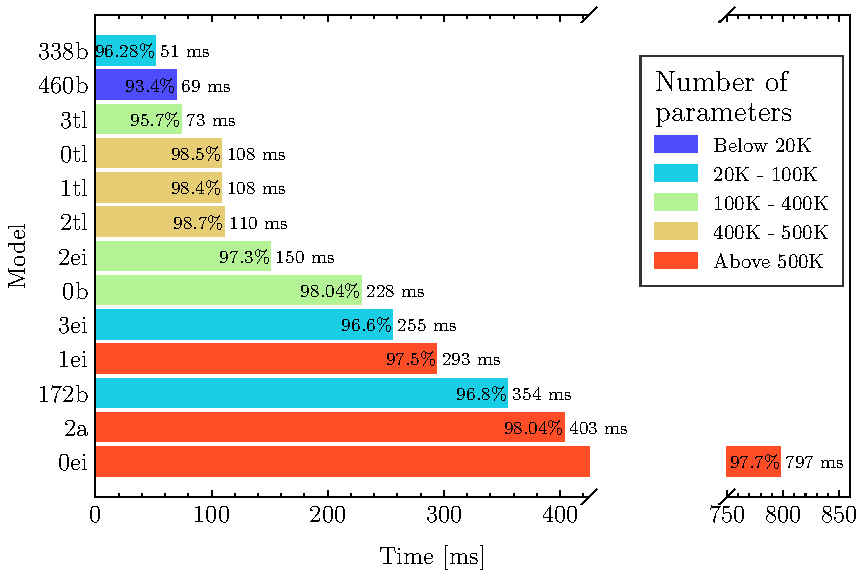
\includegraphics[width=1\linewidth]{speed_comp.pdf}
    \caption{ Comparison of time of inference of different models.}
    \label{speed_comp}
\end{figure}

We can see that all models perform inference in less than 1 second, which was a constraint that we set earlier in Section \ref{model_obj}.
Best time wise performing model was \textit{338b} with inference time of 51 \si{\milli\second}, there are also many models that perform inference under 300 \si{\milli\second}.

We also discovered some unexpected trend in results.
We assumed that inference time is proportional to the number of parameters if the general structure of the model remains the same.
As can be seen in Figure \ref{speed_comp} there are few exceptions to this rule, model \textit{338b} executed inference faster than \textit{460b} although it has more parameters (20K versus 13K).
Model \textit{172b} was slower than \textit{0b}, although it has five times less parameters.
This behaviour is not exclusive only to our models, but it can be seen in Edge Impulse models as well, for example, models \textit{2ei} and \textit{1ei}.

Edge Impulse models trained with Transfer Learning technique \textit{0tl}, \textit{1tl}, \textit{2tl} and \textit{3tl} should not be compared to other models in this sense, as the architecture of MobileNetV2 contains additional different operations.

We can only speculate about the reason for this behaviour, since it is present both in our models and Edge Impulse models, we can assume this to be a TFLite bug.

\subsection{ Comparison of code sizes}

We also wanted to inspect Flash and RAM sizes of binaries, that we compiled for on-device testing.
For this task we used \verb|arm-none-eabi-size| command line tool which returns sizes of \verb|text|, \verb|data|, \verb|bss| sections in bytes, example of output can be seen in Figure \ref{size_output}.
To compute used Flash we need simply add bytes from \verb|text| and \verb|data| sections, and to compute used RAM we add together \verb|data| and \verb|bss| sections\footnotemark.
\lstset{style=mystyle}
\begin{figure}[ht] 
\begin{lstlisting}[language=bash]
$ arm-none-eabi-size firmware.elf
   text	   data	    bss	    dec	    hex	filename
 149124	    388	  47064	 196576	  2ffe0	firmware.elf
\end{lstlisting}
\captionof{lstlisting}{ Example output of arm-none-eabi-size command.}
\label{size_output}
\end{figure}
\footnotetext{ Data section which contains initialized static variables is first placed into Flash memory and is copied to RAM before program enters main function. That is why we have to account for additional \verb|data| section in Flash memory.}
Code sizes for all models are presented in Figure \ref{size_comp}, models are ordered the same way as they have been in Figure \ref{speed_comp}.
\begin{figure}[ht]
    \centering
    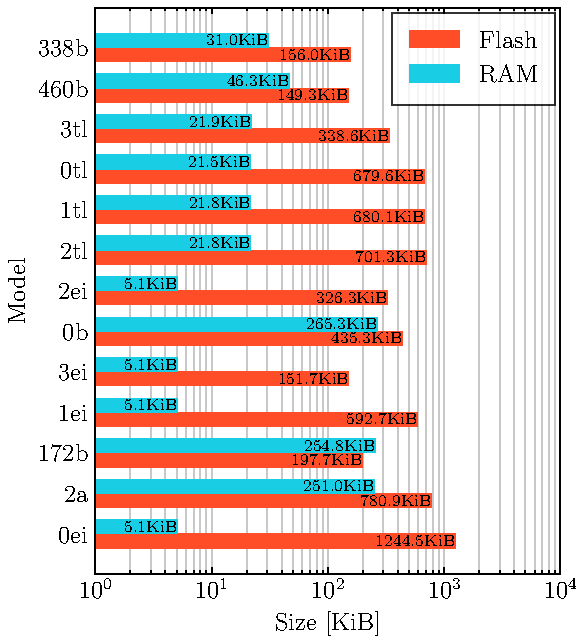
\includegraphics[width=1\linewidth]{size_comp.pdf}
    \caption{ Comparison of Flash and RAM size of compiled example models.}
    \label{size_comp}
\end{figure}

We can see that all of our models generally use more RAM then edge Impulse models.
This is due to how the inference is executed.
TFLite Micro uses a generic interpreter approach, where the model is loaded at runtime.
Edge Impulse uses a compiled approach, which they named The EON\textsuperscript{TM} Compiler\cite{eon}.
The EON\textsuperscript{TM} Compiler still uses TFLite Micro, however, it does not use its interpreter, but directly calls operation kernels.
This means that linker knows exactly which operations are used and more data can be moved into Flash, thus eliminating unneeded code size\cite{eon}.


\subsection{ Comparison of different optimisations}

To be able to run the ML inference at maximum possible efficiency under MicroML some extra amount of work and research was required.
Figure \ref{opt_comp} shows reductions in inference time of \textit{0b} model while using different optimisation methods.
\newline

\begin{figure}[ht]
    \centering
    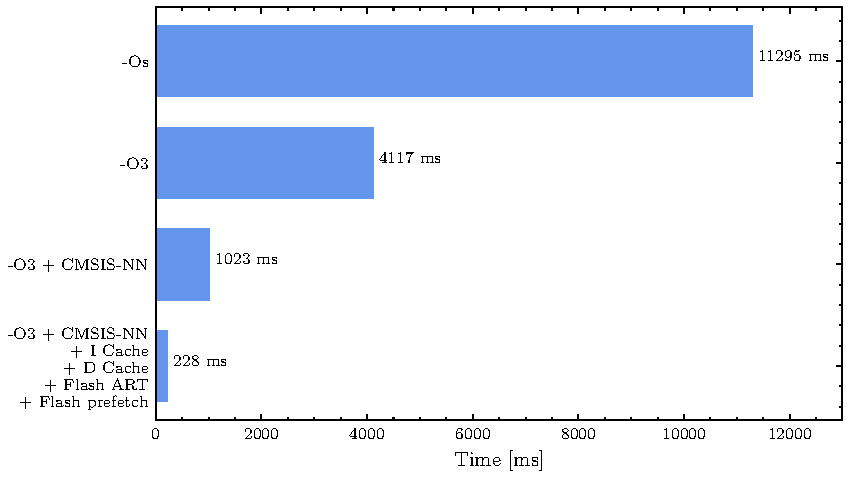
\includegraphics[width=1\linewidth]{opt_comp.pdf}
    \caption{ Inference time of \textit{0b} model using different optimisations.}
    \label{opt_comp}
\end{figure}

We started with no optimisations at all, while using only \verb|-Os| compiler flag.
\verb|-Os| flag generally optimises for minimal size, it enables all \verb|-O2| optimisations, except those that increase size.
This optimisation level is often used, however, we found out that inference time of more than 11 seconds was too long.

Changing optimisation level to \verb|-O3| drastically decreased the time of inference, down to 4117 \si{\milli\second}.
\verb|-O3| turns on all \verb|-O2| optimisations plus additional ones and completely disregards any code size optimisations.

Changing compiler optimisations flags could not lower time of inference any further, so other approaches were needed.
While reading through TensorFlow documentation we saw that it supports CMSIS-NN library for ARM microcontrollers.
CMSIS-NN is a collection of efficient Neural Network kernels, that intends to maximise performance and lower code size of NN models implemented on ARM microcontrollers.
TensorFlow provides wrappers for some of these kernels, such as convolutional, fully connected, pooling layers and others.
Not much work was needed to use these highly efficient kernels, we only needed to specify in our Makefile that we want to compile CMSIS-NN kernels and not compile generic TensorFlow kernels. 
Time of inference dropped for about 3 seconds, down to 1023 \si{\milli\second}.

As we saw that similarly sized Edge Impulse models were running much faster on Mbed platform compared to our MicroML code, while using the same microcontroller, we knew that there was another step left.
The final performance increase was reached by using features only fully found in Cortex-M7 microcontrollers and partly in Cortex M3/4 microcontrollers. 
To achieve it we had to enable I and D caches, flash prefetch and flash ART.

ART stands for Adaptive real-time memory accelerator, which encompasses I/D caches and flash prefetch buffer.
I and D caches are small, efficient portions of memory, which are located in the CPU of the microcontroller.
They hold instructions and data respectively, if those are requested by next microcontroller instruction, they can be read much faster compared to reading them from flash memory. 
By enabling flash prefetch microcontroller reads additional sequential instructions into prefetch buffer, thus enabling execution without any wait states (if instruction flow is sequential).
Elimination of wait states greatly improved the time of inference, it was decreased to 228 \si{\milli\second}.


\subsection{ Scoring trained models}\label{scoring_models}

Choosing the best model for on-field deployment is a hard task due to many different metrics: precision and recall values, time of inference, and code size.
To make this job easier we devised a scoring system: each metric is going to be normalized and multiplied with some weight value.
All products would then be summed up and the result would represent the final score.
The sum of the weights is equal to 100, which means that the possible maximum score is also 100.
We decided to allocate 50 weight points to all precision and recall values, 30 points to the time of inference value, 5 points for Flash size and 15 points for RAM size.
As we care more about precision and recall values of elephant, human and cow classes we gave them 7 weight points each, while nature/random class received only 4.
We value Flash size less than RAM, as most of the microcontrollers have much less RAM than they do Flash, thus we gave 15 weight points to RAM size and only 5 to Flash size.

Since the time of inference, Flash and RAM sizes are properties, which should give a larger score, the smaller they are, we mapped them into a range between 0 and 1.
The smallest value inside the set would be assigned 1, the biggest 0, the values in between are mapped linearly.

Scoring is described mathematically in \ref{score_equ}, while the final results can be seen in Figure \ref{score_comp}.
\begin{equation}\label{score_equ}
    \begin{aligned}
        Score[i] ={} & 7 K(P_{elephant},i) + 7 K(P_{human},i) + 7 K(P_{human},i) + 4 K(P_{ntr/rnd},i) \\
                     & +{} 7 K(R_{elephant},i) + 7 K(R_{human},i) + 7 K(R_{human},i) + 4 K(R_{ntr/rnd},i) \\
                  & +{} 30\: F(ToI, i) +5\: F(Flash, i) + 15\: F(RAM, i)   \\
                  & \\
        K(X, i) ={}  & \frac{(X[i] - MIN(X))}{MAX(X)- MIN(X)} \\
                  & \\
        F(X, i) ={}  & \frac{(X[i] - MAX(X))}{MIN(X)- MAX(X)}
    \end{aligned}
\end{equation}
\clearpage
Where:\\
$Score$ - Vector of calculated scores\\
$i$ - i$^{th}$ model\\
$P_{j}$ - Vector of precision values of j$^{th}$ class\\
$R_{j}$ - Vector of recall values of j$^{th}$ class\\
$ToI$ - Vector of Time of Inference values\\
$Flash$ - Vector of Flash sizes\\
$RAM$ - Vector of RAM sizes\\
$K(X,i)$ - Normalizing function with vector X and element index i as arguments\\
$F(X,i)$ - Normalizing, inverting, function with vector X and element index i as arguments\\
$MAX(X)$ - Function that finds maximum element in vector X\\
$MIN(X)$ - Function that finds minimum element in vector X

\begin{figure}[ht]
    \centering
    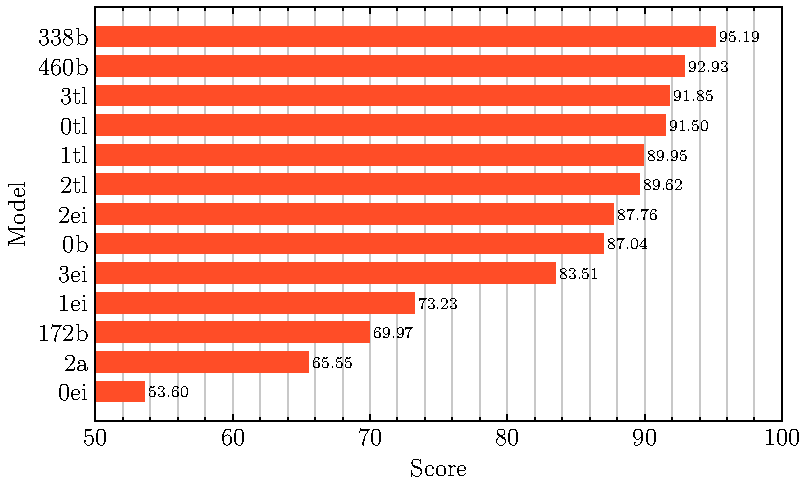
\includegraphics[width=1\linewidth]{score_comp.pdf}
    \caption{ Score comparison of different models}
    \label{score_comp}
\end{figure}

\section{ Summary of model testing}

As we saw in Figure \ref{score_comp} model \textit{3tl} received the highest score, models \textit{1tl}, \textit{2tl} follow.
This should not be a surprise, models trained with Transfer Learning achieved high accuracies and executed inference in about 100 \si{\milli\second}. 
Additionally, compiled approach for computing Neural Networks keeps used Flash and RAM sizes to a minimum.
We saw that using a number of different optimisations is critical to achieving low inference times, thus making ML on embedded device viable.

\section{ Power profiling of an embedded early warning system}

\subsection{ Measuring setup}

To measure power consumption we used product called Otii Arc (Otii), which can be seen in Figure \ref{otii}.
Otii, made by a company Qoitech, is a small portable box, that contains a power supply, a current and voltage measurement unit and a data acquisition module.
It connects to a computer over USB cable and can be powered through it or with an external charger.

It can provide output voltage between 0.5 V and 4.55 V and has accuracy of $\pm$(0.1 \% + 50 nA), when measuring current.
It is a perfect tool for evaluating low-power systems.
\newline
\begin{figure}[ht]
    \centering
    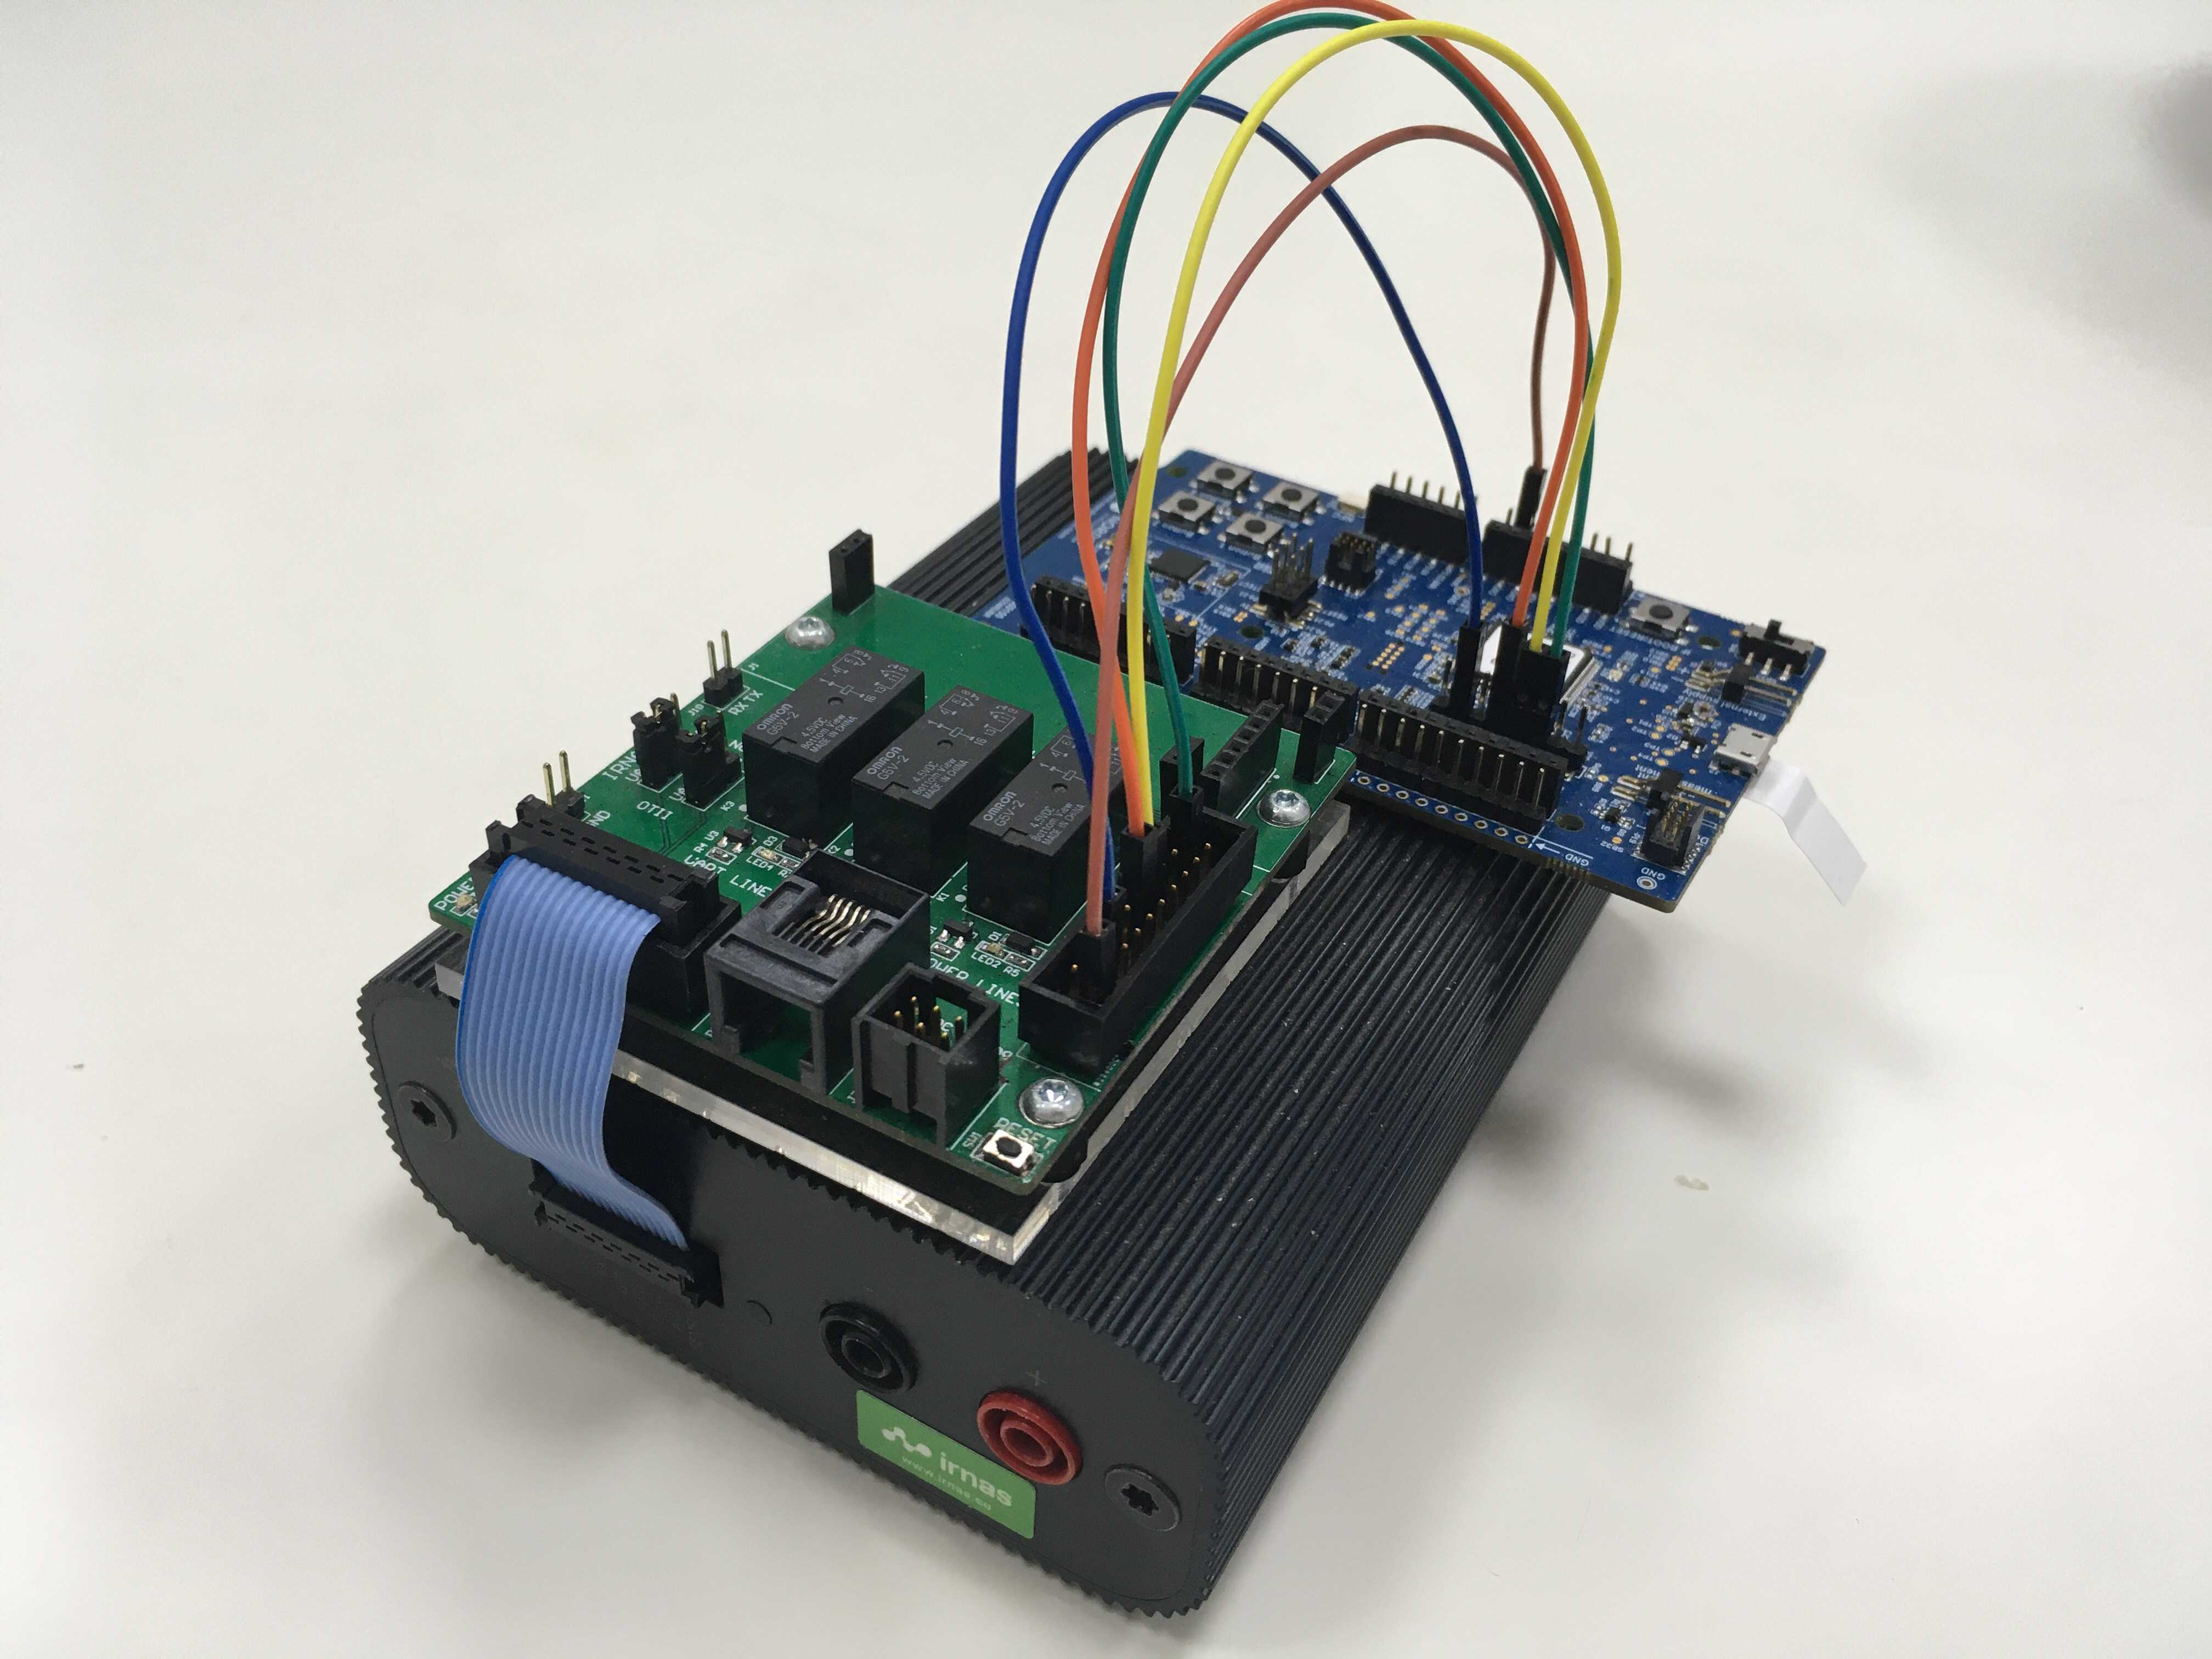
\includegraphics[width=0.75\linewidth]{otii.jpg}
    \caption{ Otii Arc with nRF52832 DK and added measurement board made by IRNAS.}
    \label{otii}
\end{figure}

Measurements analysis is done through desktop application, example of it is seen in Figure \ref{otii_screen}. 
Application enables users to select a part of the measurement, for which it automatically computes minimum, maximum and average values.
To present our results we exported current measurements in CVS format and plotted them with Matplotlib.
\newline
\begin{figure}[ht]
    \centering
    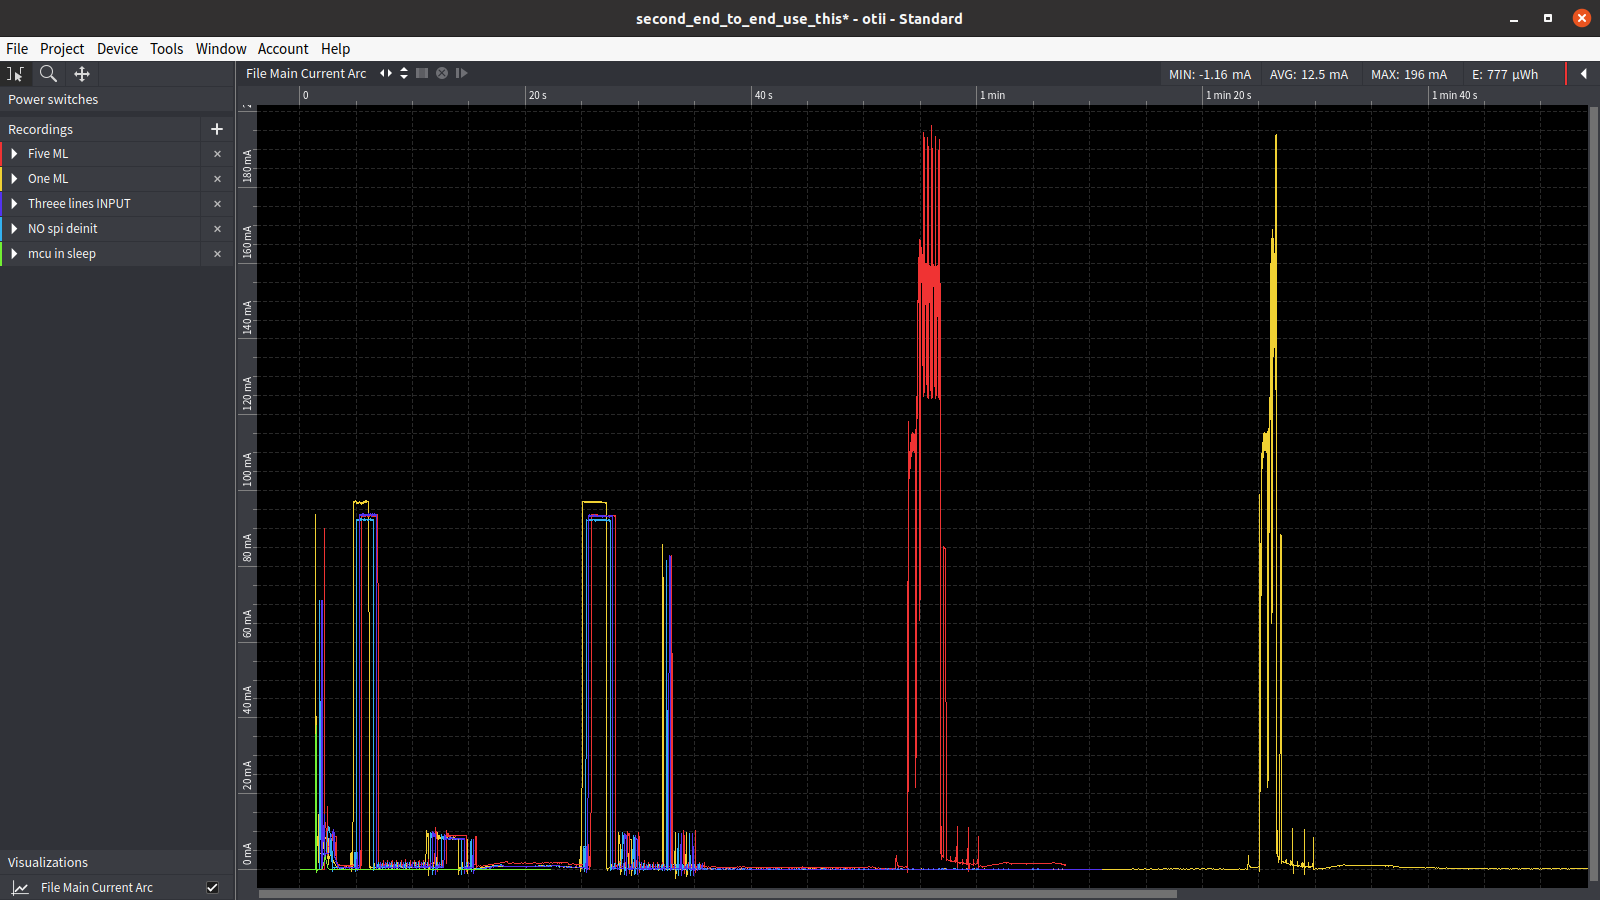
\includegraphics[width=1\linewidth]{otii_screenshot.png}
    \caption{ Screenshot of Otii user interface.}
    \label{otii_screen}
\end{figure}

In the next section we evaluate power consumption of our embedded early warning system.
We first measured power consumption of the nRF52 microcontroller in low-power state, then we connected the LR1110 evaluation shield to the nRF52840 DK board and repeated the measurement.
We then connected Nucelo-F767ZI and FLIR camera, and measured power consumption of the whole detection sequence.


\subsection{ Current measurements}

We conducted all our measurements with Otii's output voltage set to 3.3 V.
Before measuring current consumption of the whole image processing sequence we wanted to evaluate current consumption of nRF52 microcontroller in the low-power state.
In Zephyr kernel such procedure is relatively simple, type of sleep mode is configured with Kconfig file and microcontroller transitions into it whenever it enters lowest idle thread.
Peripherals require special attention, as needs to be explicitly specified which one needs to be turned off.
We turned off both of the UART peripherals and SPI peripheral, while keeping GPIO active, as we needed a GPIO interrupt to wakeup nRF52 from low-power state.
We also had to make sure that nRF52 microcontroller is completely disconnected from on board J-Link debug probe to avoid any unnecessary current leaks.
Luckily the nRF52840 development board has an analogue switch, which does exactly that.
To measure current consumption we simply connected voltage output of Otii to external power pins of nRF52840 DK board.
Figure \ref{mcu_in_sleep} shows the current consumption in the low-power state.
\newline
\begin{figure}[ht]
    \centering
    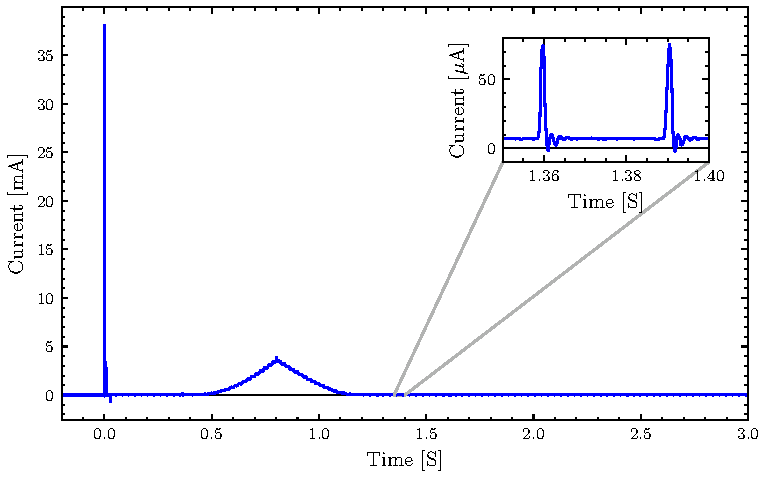
\includegraphics[width=1\linewidth]{mcu_in_sleep.pdf}
    \caption{ Current consumption of nRF52840 microcontroller in low-power state.}
    \label{mcu_in_sleep}
\end{figure}

Initial spike at the beginning of graph happens due to many decoupling capacitors on the board.
Due to the sudden change in voltage their impedance is low, therefore more current is drawn.
Pyramid looking shape between 0.5 and 1 second happens due to the onboard regulators turning on.

Smaller graph inside Figure \ref{mcu_in_sleep} shows close up view of the current consumption.
The peaks reached 70.3 \si{\micro\ampere}, steady state was at 6.9 \si{\micro\ampere}, while the average was 9.1 \si{\micro\ampere}.
Peaks were repeating at frequency of 33.3 \si{\hertz}.

Measured average current was higher than expected, according to the nRF52's datasheet\cite{nrf52_datasheet} current consumption should be 3.16 \si{\micro\ampere}.

In next measurement we connected LR1110 shield to the nRF52840 DK board and observed current consumption of the initial LoRaWAN join sequence.
Current profile of it can be see in Figure \ref{lora_join}.
\newline
\begin{figure}[ht]
    \centering
    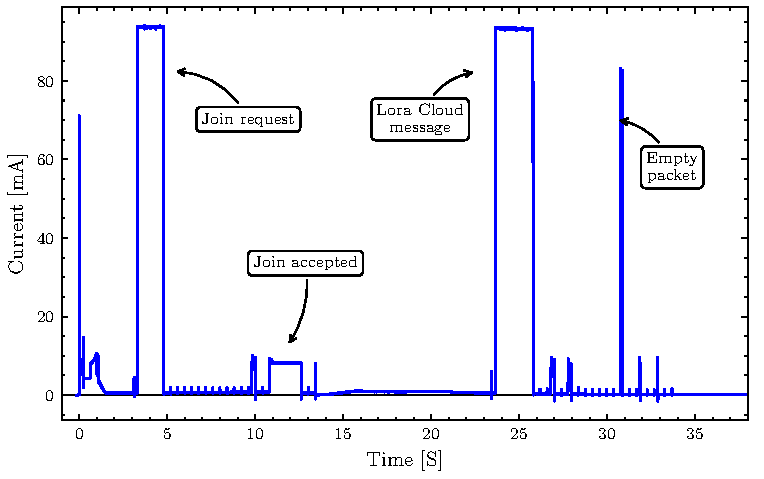
\includegraphics[width=1\linewidth]{lora_join.pdf}
    \caption{ Current profile of LoRaWAN join sequence.}
    \label{lora_join}
\end{figure}

Besides initial spike we can see additional four pulses afterwards with some smaller spikes in between. 
As we are using Over-The-Air Activation (OTAA) LR1110 first has to negotiate for a set of keys with the server before it can start transmitting.
This happens in first two pulses, LR1110 first sends join request and then listens for response.
After receiving response it confirms it.
In third pulse LR1110 sends a message that is a part of the LoRa Cloud service.
This message is specific to LR1110 and it can not be completely disabled.
Last thin pulse belongs to an empty payload message, which LR1110 always transmits in beginning.
Average current consumption of LoRaWan join procedure is 11.4 \si{\milli\ampere} and lasts for about 34 seconds.
Average current consumption in sleep state has increased to 76.8 \si{\micro\ampere}.

In our next test we connected nRF52 to boost converter circuit, Nucleo-F767ZI and FLIR Lepton camera, setup can be seen in Figure \ref{measure_setup}.
We did not use PIR sensor as a wakeup source as we saw that its detection was too sensitive to surroundings and we could not completely control it.
We instead used a button on nRF52840 DK as a wakeup interrupt.
To account for PIR sensor current consumption in later calculations we measured it separately, we saw that it drew 130 \si{\micro\ampere}.
\newline
\begin{figure}[ht]
    \centering
    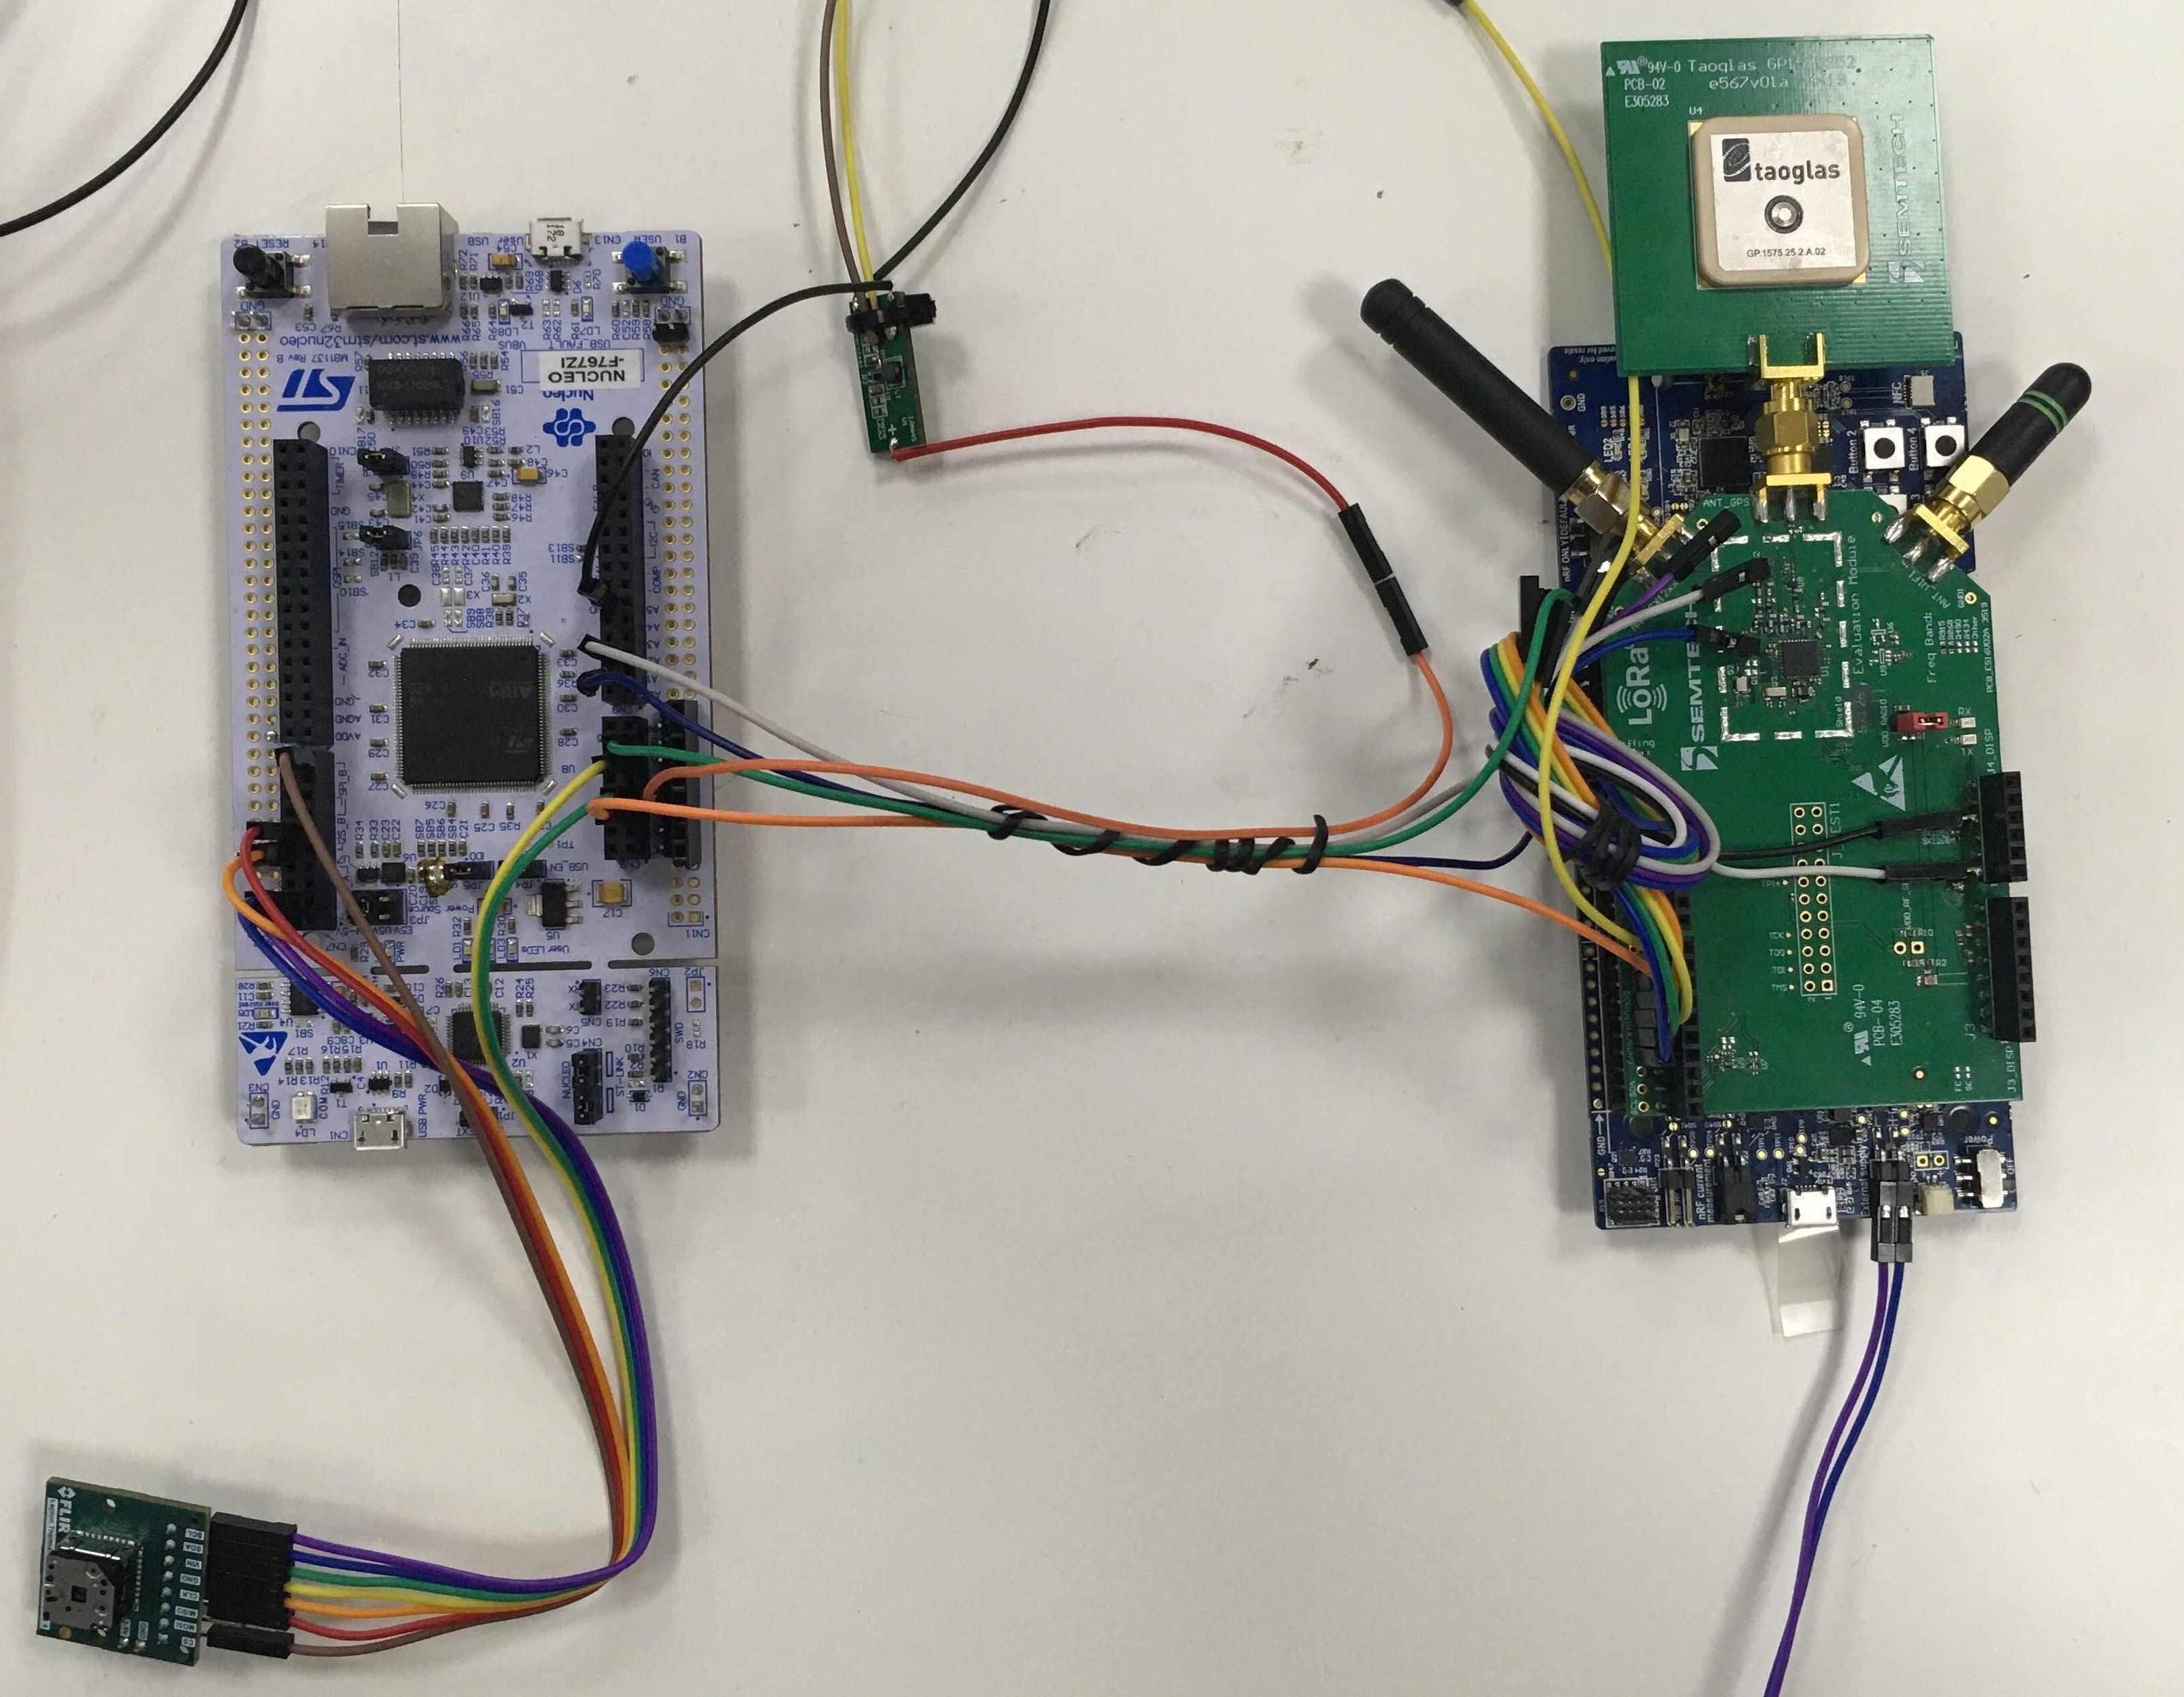
\includegraphics[width=0.75\linewidth]{measure_setup.jpg}
    \caption{ Device under test: nRF52840 DK with attached LR1110 shield, boost converter breakout board, Nucleo-F767ZI and FLIR Lepton camera.}
    \label{measure_setup}
\end{figure}

Since we wrote our firmware for libopencm3 in mind we could not use the best performing model \textit{3tl}, as Edge Impulse models only could run on Mbed platform.
We instead used our model \textit{460b}, as was most similar to \textit{3tl} in terms of inference time (69 \si{\milli\second} compared to 73 \si{\milli\second}).
We captured two different inference procedures, in first image capture and inference were done once, in second one they were repeated 5 times.
Procedures can be seen on Figures \ref{one_ml} and \ref{five_ml} respectively.
Both procedures were followed by a LoRaWAN message that reported results to the server.
\begin{figure}[ht]
    \centering
    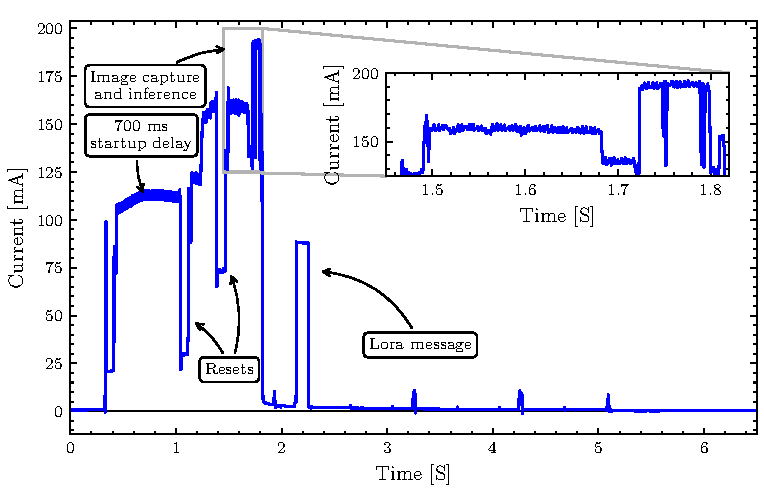
\includegraphics[width=1\linewidth]{one_ml.pdf}
    \caption{ Current profile of image capture and inference procedure.}
    \label{one_ml}
\end{figure}
\begin{figure}[ht]
    \centering
    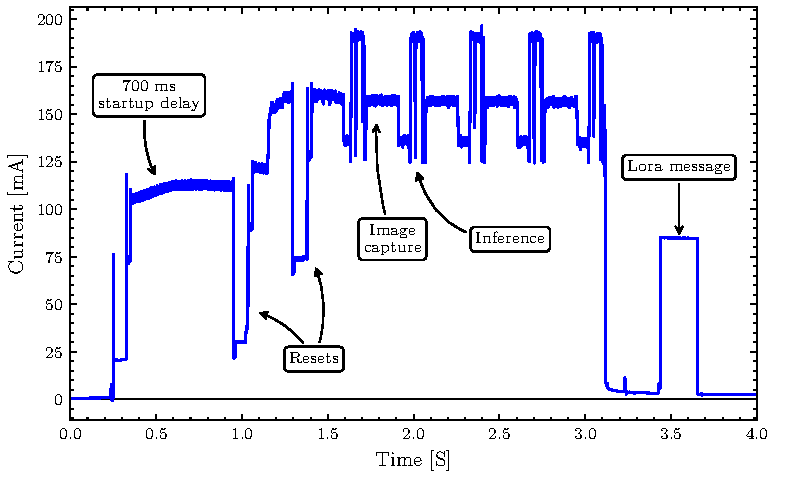
\includegraphics[width=1\linewidth]{five_ml.pdf}
    \caption{ Current profile of image capture and inference procedure repeated 5 times.}
    \label{five_ml}
\end{figure}
\clearpage
In case where image capture and inferencing happened once, we measured total time of the whole detection procedure to be about 1480 \si{\milli\second}, not including the time needed for LoRaWAN message.
Average current consumption for this period was 114 \si{\milli\ampere}.
Measured average current of the whole event shown on Figure \ref{one_ml}, between 0 and 6 seconds, is 30 \si{\milli\ampere}.

In case where image capture and inferencing happened five times, we measured total time of the whole detection procedure to be about 2960 \si{\milli\second}, not including time needed for LoRaWAN message.
Average current consumption for this period was 131 \si{\milli\ampere}.
If we add transmission of LoRaWAN message to the measured current consumption, thus increasing the time of the whole detection event to 8 seconds, we measure 51.9 \si{\milli\ampere}.



\subsection{ Commentary of the current measurement results}

Measured low-power state of nRF52, visible in Figure \ref{mcu_in_sleep}, was higher than expected.
nRF52's datasheet\cite{nrf52_datasheet} specifies current consumptions in many different conditions, which depend on: type of sleep mode (System ON or System OFF, latter loses execution context at wakeup), amount of RAM retention and type of wakeup event.
Consumption can range from 0.95 \si{\micro\ampere} to 17.37 \si{\micro\ampere}.
Because Zephyr provides only abstract interface to power management, implementation of which is platform dependant, we can only guess which exact nRF52 sleep mode Zephyr uses.
We assumed expected current consumption of 3.16 \si{\micro\ampere} as this is the specified current consumption in System ON mode with full RAM retention and LFRC set as a wakeup event.
Another reason for increased power consumption could also be inadequate support circuitry of nRF52840 DK board.

When we connected LR1110 shield to the nRF52840 DK board we saw that average current consumption increased to 76.8 \si{\micro\ampere}, which is much more than expected.
LR1110 automatically enters sleep mode when it is finished with communication, according to its datasheet\cite{lr1110_datasheet}, current consumption should be around 1.85 \si{\micro\ampere}.
This current consumption is plausible, as we observed it in other IRNAS's products that use LR1110 chip.
We suspect that the incorrect state of common GPIO connections between LR1110 and nRF52 is the reason for increased current consumption, however we were not able to fix the problem.

We mentioned that the time required for detection is about 1480\si{\milli\second}, if we capture one image and process it or 2960 \si{\milli\second}, if done five times.
We can see that both detection procedures started with a 700 \si{\milli\second} of delay, according to FLIR Lepton's datasheet \cite{flir_datasheet}, a delay is required before we can start communicating with the camera over TWI interface.
Two microcontroller resets are visible, during our testing we saw that we could not properly communicate with the camera, if we did not reset STM32 twice before that.
To accomplish this we simply connected a reset pin of STM32 with one of available nRF52 GPIO pins.


\subsection{ Battery life estimations}

Table \ref{lifetime_data} shows parameters values that we used in our equation \ref{lifetime_equ} of battery lifetime.
We define a detection sequence where image capture and inference are repeated 5 times and then followed by a LoRaWAN message.
In our calculation we also accounted for one daily LoRaWAN message, which is meant for system reporting.
We assumed that system is in low-power mode when is not performing detection sequence or sending a LoRaWAN message.
As a power source we chose a lithium-ion cell battery NCR 18650B of manufacturer Panasonic.
Its properties can be seen in Table \ref{lifetime_data}.

\begin{table}[ht]
    \centering
    \caption{ First hyperparameter search space}
    \rowcolors{2}{white}{gray!25}
    \begin{tabular}{lr}    \toprule
        \textbf{Event}                          & \textbf{Current consumption at 3.3 V} \\\midrule
        low-power state                         & 76.8\si{\micro\ampere}                \\ 
        PIR                                     & 130\si{\micro\ampere}                 \\ 
        PIR and low-power state                 & 206.8\si{\micro\ampere}               \\
        Detection sequence, 8 s                 & 51.9\si{\milli\ampere}                \\
        LoRaWAN message, 230 \si{\milli\second} & 80 \si{\milli\ampere}                 \\\midrule
        \textbf{Battery type}                   & \textbf{Properties}                   \\
        Panasonic NCR 18650B                    & Nominal Voltage: 3.6 V                \\
                                                & Nominal Capacity: 3350 \si{\milli\ampere\hour}\\\bottomrule
    \end{tabular}
    \label{lifetime_data}
\end{table}

\begin{equation}\label{lifetime_equ}
\begin{aligned}
    P_{sleep} ={} & U_{supplied}\; I_{sleep}\\
P_{detect} ={} & U_{supplied}\; I_{detec}\\
P_{lora} ={} & U_{supplied}\; I_{lora}\\
t_{sleep}     ={} & 24h - t_{detect}\; N_{detect} - t_{lora}\\
P_{average}   ={} & \frac{P_{sleep}\; t_{sleep} + P_{detect}\;t_{detect}\; N_{detect} + P_{lora}\; t_{lora}}{24h}\\
t_{lifetime}  ={} & \frac{U_{bat}\;Ah_{bat}\;N_{bat}}{P_{average}}
\end{aligned}
\end{equation}

Where:\\
$U_{supplied}$ - Voltage at which we have done our measurements, 3.3 V\\
$U_{bat}$ - Battery nominal voltage, 3.6 V\\
$Ah_{bat}$ - Battery nominal capacity, 3350 \si{\milli\ampere\hour}\\
$I_{lora}$ - Current consumption when sending a LoRaWAN message\\
$I_{sleep}$ - Current consumption of low-power state with PIR consumption\\
$I_{detect}$ - Current consumption of detection sequence\\
$P_{sleep}$ - Used power of low-power state and PIR\\
$P_{detect}$ - Used power of detection sequence\\
$P_{lora}$ - Used power of LoRaWAN message send\\
$P_{average}$ - Average power needed for system to operate\\
$t_{detect}$ - time spent in detection sequence in hours\\
$t_{sleep}$ - time spent in low-power state in hours\\
$t_{lora}$  - time spent sending LoRaWAN messages\\
$t_{lifetime}$ - battery life time in hours\\
$N_{detec}$ - Number of detection in a day\\
$N_{bat}$ - Number of batteries

Because we can only assume how frequently will our system need to perform detection sequence, we repeated our calculation for several different numbers of detections per day.
We also varied the number of battery cells, the enclosure, that we plan to use, has enough space for up to 6 battery cells.
Results of the estimations can be seen in Figure \ref{lifetime_figure}, X axis represents number of battery cells, Y axis represents system life time in months and the colour of the lines represents number of detections per day, from 100 to 600.

\begin{figure}[ht]
    \centering
    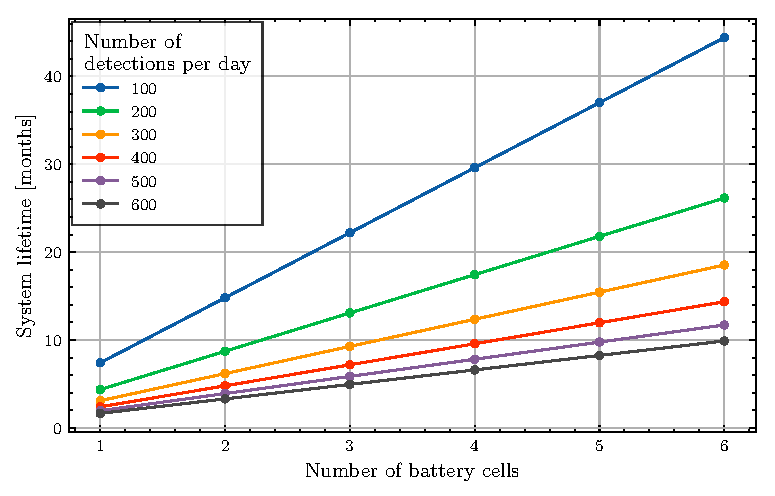
\includegraphics[width=1\linewidth]{lifetime.pdf}
    \caption{ Current profile of image capture and inference procedure.}
    \label{lifetime_figure}
\end{figure}

Results are promising, we can see that most battery configurations last more than 6 months, which is already a long time, considering the application.
If decide on 6 battery cell configuration, we see that in worst case where we are executing 600 detection per day, we can expected system lifetime of 10 months, which is more than enough.
There are some things that we have to take into account.
We assumed 100 \% battery efficiency, meaning that each battery will provide its complete nominal capacity, in our case 3350 \si{\milli\ampere\hour}.
In practice this is not possible due to effects such as self-discharge rate, high discharge profiles and temperature influences.
On the other hand we assumed that we will process same amount detections everyday, in worst case 600.
This number is probably much, and actual system lifetime should be better.

While calculating system lifetime, we tried changing input parameters to see which ones affect final lifetime of the system the most.
We found out that by decreasing current consumption in low-power state by ten times (from 206.8 \si{\micro\ampere} to 21 \si{\micro\ampere}) we do not dramatically increase the system's lifetime.
With 6 batteries and 600 detections per day the lifetime increased to 10.5 months from 9.9 months.
However, we saw large increase in system's lifetime if we halved either current consumption of detection event or its duration, with same conditions as before the system's lifetime increased from 9.9 to 18.5 months.
This means that in order to increase systems's lifetime or to keep it the same with smaller number of batteries, we should focus on lowering the power consumption of detection event than lowering the low-power state current.


% Include bibliograpfy and justify it right. Use myunsrt biblio style.
\begingroup
\raggedright
\bibliographystyle{myunsrt}
\bibliography{chapters/literature}
\endgroup
\end{document}

